%
% The first command in your LaTeX source must be the \documentclass command.
%\documentclass[sigconf,review,anonymous,dvipsnames]{acmart}
\documentclass[sigconf]{acmart}

\usepackage{listings}
\usepackage{multirow}
\usepackage{lscape}
\usepackage{amsmath}
\usepackage{amsthm}
\usepackage{tikz}
\usetikzlibrary{shapes,arrows}
\usepackage{graphicx}
\usepackage[T1]{fontenc} 
\usepackage[scaled=0.80]{beramono}
\usepackage{graphicx} % http://ctan.org/pkg/graphicx
\usepackage{booktabs} % http://ctan.org/pkg/booktabs
\usepackage{xparse}
\usepackage{adjustbox}
\usepackage{subcaption}
%\usepackage{showframe}

\renewcommand{\dblfloatpagefraction}{0.5} % allow float page
\def\sectionautorefname{Section}
\def\subsectionautorefname{Section}

\usepackage[backgroundcolor=Apricot, textsize=footnotesize]{todonotes}
\newcommand*{\eva}[1]{\todo[author=Eva,inline,caption={}]{#1}}
\newcommand*{\rocco}[1]{\todo[author=Rocco,inline,caption={}]{#1}}

\newcommand{\Sadegh}{\textcolor{blue}}
\newcommand{\Mahmoud}{\textcolor{magenta}}
\newcommand{\Mahmoudd}{\textcolor{blue}}
\newcommand{\RM}[1]{{\textcolor{red}{$\clubsuit$ #1 $\clubsuit$}}}
\newcommand{\Eva}{\textcolor{green}}
\newcommand{\Rocco}{\textcolor{brown}}

\newcommand{\statevar}{x_{k}}
\newcommand{\statevarmath}{$x_{k}\,$}
\newcommand{\qstatevar}{\hat{x}_{k}}
\newcommand{\qstatevarmath}{$\hat{x}_{k}\,$}
\newcommand{\statespace}{X}
\newcommand{\regioni}[1]{$X_{{#1}}$}
\newcommand{\regionimath}[1]{X_{{#1}}}
\newcommand{\maxUij}{$max|U_{i}-U_{j}|$}
\newtheorem{remark}{Remark}

\usepackage{sansmath}
\newcommand{\inputm}[1]{\mathsf u_{{#1}}}

\def\equationautorefname~#1\null{%
  Equation~(#1)\null
}
% Rights management information. 
% This information is sent to you when you complete the rights form.
% These commands have SAMPLE values in them; it is your responsibility as an author to replace
% the commands and values with those provided to you when you complete the rights form.
%
%These commands are for a PROCEEDINGS abstract or paper.
%\copyrightyear{2018}
%\acmYear{2018}
%\setcopyright{acmlicensed}
%\acmConference[Woodstock '18]{Woodstock '18: ACM Symposium on Neural Gaze Detection}{June 03--05, 2018}{Woodstock, NY}
%\acmBooktitle{Woodstock '18: ACM Symposium on Neural Gaze Detection, June 03--05, 2018, Woodstock, NY}
%\acmPrice{15.00}
%\acmDOI{10.1145/1122445.1122456}
% \acmISBN{978-1-4503-9999-9/18/06}

%
% These commands are for a JOURNAL article.
%\setcopyright{acmcopyright}
%\acmJournal{TOG}
%\acmYear{2018}\acmVolume{37}\acmNumber{4}\acmArticle{111}\acmMonth{8}
%\acmDOI{10.1145/1122445.1122456}

%
% Submission ID. 
% Use this when submitting an article to a sponsored event. You'll receive a unique submission ID from the organizers
% of the event, and this ID should be used as the parameter to this command.
%\acmSubmissionID{123-A56-BU3}

%
% The majority of ACM publications use numbered citations and references. If you are preparing content for an event
% sponsored by ACM SIGGRAPH, you must use the "author year" style of citations and references. Uncommenting
% the next command will enable that style.
%\citestyle{acmauthoryear}

%
% end of the preamble, start of the body of the document source.
\begin{document}

%
% The "title" command has an optional parameter, allowing the author to define a "short title" to be used in page headers.
\title{Memory-Efficient Mixed-Precision Implementations\\for Robust Explicit Model Predictive Control}

%
% The "author" command and its associated commands are used to define the authors and their affiliations.
% Of note is the shared affiliation of the first two authors, and the "authornote" and "authornotemark" commands
% used to denote shared contribution to the research.
\author{Mahmoud Salamati}
\authornote{Both authors contributed equally to this research.}
\affiliation{
	\institution{MPI-SWS}
%  \streetaddress{P.O. Box 1212}
\city{Kaiserslauterm}
\country{Germany}
%  \state{Ohio}
%  \postcode{43017-6221}
}
\email{msalamati@mpi-sws.org}
%\orcid{1234-5678-9012}


\author{Rocco Salvia}
\authornotemark[1]
\affiliation{
	\institution{University of Utah}
%  \streetaddress{P.O. Box 1212}
  \city{Utah}
  \country{United States}
%  \state{Ohio}
%  \postcode{43017-6221}
}
\email{rocco@cs.utah.edu}


\author{Eva Darulova}
\affiliation{%
  \institution{MPI-SWS}
%  \streetaddress{1 Th{\o}rv{\"a}ld Circle}
  \city{Kaiserslautern}
  \country{Germany}}
\email{eva@mpi-sws.org}

\author{Sadegh Soudjani}
\affiliation{
  \institution{Newcastle University}
  \city{Newcastle}
  \country{United Kingdom}
}
\email{sadegh.soudjani@newcastle.ac.uk}


\author{Rupak Majumdar}
\affiliation{
 \institution{MPI-SWS}
% \streetaddress{Rono-Hills}
 \city{Kaiserslautern}
% \state{Arunachal Pradesh}
 \country{Germany}}
\email{rupak@mpi-sws.org}

%
% By default, the full list of authors will be used in the page headers. Often, this list is too long, and will overlap
% other information printed in the page headers. This command allows the author to define a more concise list
% of authors' names for this purpose.
%\renewcommand{\shortauthors}{Trovato and Tobin, et al.}

\renewcommand{\shortauthors}{}

%
% The abstract is a short summary of the work to be presented in the article.
\begin{abstract}
We propose an optimization for space-efficient implementations of explicit model-predictive controllers (MPC)
for robust control of linear time invariant (LTI) systems on embedded platforms. 
We obtain an explicit-form robust model-predictive controller as a solution to a multi-parametric 
linear programming problem.
The structure of the controller is a polyhedral decomposition of the control domain,
with an affine map for each domain.
While explicit MPC is suited for embedded devices with low computational power, the memory requirements
for such controllers can be high.
We provide an optimization algorithm for a mixed-precision implementation of the controller,
where the deviation of the implemented controller from the original one is within the robustness
margin of the robust control problem.
The core of the mixed-precision optimization is an iterative static analysis that co-designs
a robust controller and a low-bitwidth approximation 
that is statically guaranteed to always be within the robustness margin to the original controller.
We have implemented our algorithm and show, on a set of Simulink benchmarks, that our optimization
can reduce space requirements by up to 20\% (and about 10\% on average), compared to a fixed precision
implementation of the original controller.


\end{abstract}

%
% The code below is generated by the tool at http://dl.acm.org/ccs.cfm.
% Please copy and paste the code instead of the example below.
%
% \begin{CCSXML}
% <ccs2012>
%  <concept>
%   <concept_id>10010520.10010553.10010562</concept_id>
%   <concept_desc>Computer systems organization~Embedded systems</concept_desc>
%   <concept_significance>500</concept_significance>
%  </concept>
%  <concept>
%   <concept_id>10010520.10010575.10010755</concept_id>
%   <concept_desc>Computer systems organization~Redundancy</concept_desc>
%   <concept_significance>300</concept_significance>
%  </concept>
%  <concept>
%   <concept_id>10010520.10010553.10010554</concept_id>
%   <concept_desc>Computer systems organization~Robotics</concept_desc>
%   <concept_significance>100</concept_significance>
%  </concept>
%  <concept>
%   <concept_id>10003033.10003083.10003095</concept_id>
%   <concept_desc>Networks~Network reliability</concept_desc>
%   <concept_significance>100</concept_significance>
%  </concept>
% </ccs2012>
% \end{CCSXML}

% \ccsdesc[500]{Computer systems organization~Embedded systems}
% \ccsdesc[300]{Computer systems organization~Redundancy}
% \ccsdesc{Computer systems organization~Robotics}
% \ccsdesc[100]{Networks~Network reliability}

%
% Keywords. The author(s) should pick words that accurately describe the work being
% presented. Separate the keywords with commas.
\keywords{model-predictive control, robustness, fixed-point arithmetic}


\maketitle

% !TEX root = main.tex
\section{Introduction}
\eva{General comment: it feels a bit long until the intro discusses the actual problem,
but it reads nicely and motivates the problem well, so it's probably fine}
\eva{General comment: should we add some more references to related work (and not only to MPC)?}
Model predictive control (MPC) is a technique to design control actions by solving finite-horizon open-loop
optimal control problems at each sampling instant.
The result of each optimization gives a sequence of optimal control actions, only the first of which is applied
to the process.
The same procedure is applied in the next time instant with a shifted time horizon and a new initial state, 
after receiving the updated values of the process state.
The optimization problem in MPC uses a dynamic model of the process, encodes all input and output (state) constraints, and 
optimizes a performance index. 
MPC has shown to be successful in a wide variety of industrial applications, due to its 
ability to systematically handle processes with many state and input variables as well as constraints on them. 

The main difference between MPC and conventional control is in the nature of the function that maps the measured outputs to control actions. 
MPC computes such a function \emph{online}, whereas a conventional controller pre-computes the function offline.
The online computations required in MPC limits its applicability to slow processes and fast computation platforms: 
the sampling time has to be large enough and the platform fast enough to allow enough time for solving the optimization problem
and obtaining the optimal action for the next time instance. 
Moreover, the optimization solver needs to be certified when using MPC in safety critical applications.

One way to tackle these problems is through \emph{explicit MPC} \cite{Bemporad:2002,Alessio2009}, which formulates the optimization
problem but computes offline a symbolic representation of the solution as a function of the state.
At run-time, the solution is evaluated on the current state as in conventional control.
For example, for linear time invariant models with linear constraints and quadratic costs, the optimization
problem for MPC can be modeled as a quadratic program, and explicit MPC techniques solve the optimization problem
using multi-parametric programming techniques.
The explicit solution is representable as a partition of the controller domain into a number of polyhedral regions,
and an affine map for each region.
The implementation of explicit MPC stores a lookup table of the affine maps and performs a number of affine computations
online to find the appropriate region for the current state and to evaluate the control.  
Explicit MPC thus expands the class of systems being controlled by MPC strategies, by taking out the need to compute fast online
or to certify a complex optimization routine.

However, there are still bottlenecks in implementing explicit MPC on resource-constrained embedded micro-controllers.
First, implementations of explicit MPCs can suffer from large memory usage, because the solution of the optimization
problem can involve many (often hundreds) of regions.
Since the memory consumption grows linearly with the number of regions, 
this can be a limited factor in using explicit MPC on resource-constrained micro-controllers.
Second, many low-end micro-controllers only support fixed-point arithmetic.
Errors in the controller implementation are inversely proportional to the number of bits used for representing each variable. 
An implementation of explicit MPC has to be \emph{robust} to 
implementation errors to be able to enforce hard constraints on the states at run time.

In this paper, we consider the problem of implementing explicit MPC on low-end microcontrollers with fixed-point arithmetic
in a \emph{memory-efficient} and \emph{robust} way.
We propose an automatic controller and mixed-precision implementation co-design technique that computes a minimal set \todo{What is meant by minimal?} of mixed
precision assignments for all variables while ensuring the resulting implementation error remains within the robustness margin.  


Our proposed method iteratively solves a robust version of the MPC which explicitly considers fixed-point implementation errors
in the model; see~\autoref{fig:overview}.
Initially, we estimate a bound $\Delta = \Delta_0$ on the implementation error and solve a
min-max quadratic program for explicit robust MPC \cite{delaPea:2005}, where the system
model has an explicit disturbance bounded by $\Delta$.
The solution is represented as a piecewise affine map.
We use an automated mixed-precision tuning tool to find an approximate implementation of the piecewise affine
map. 
We statically compute the error of the implementation, taking into account errors
in evaluating the affine maps as well as choosing the wrong affine map due to quantization.
If the error is at most $\Delta$, we are done: the implementation satisfies the robustness margin in the model.
If not, we increase the error bound $\Delta$ and run the loop again to find a new robust controller and find its best mixed-precision
implementation.

We have implemented our algorithm on top of Matlab's multi-parametric toolbox 
for robust explicit MPC \cite{Matlab-MPT?}
and the Daisy tool for multi-precision tuning and fixed-point error analysis \cite{Daisy}.
We have applied our technique on a number of standard benchmark examples.
Our implementation finds that our mixed-precision implementation can save up to 20\% memory (on average, XXX\%) in controller
implementations over a uniform-precision implementation (and a saving of XXX\% over a uniform 32-bit implementation), while
maintaining the correctness of the controller.
In absolute terms, the saving corresponds to YYY KB over a uniform precision implementation on our largest benchmark.
In each case, the analysis takes only a few minutes of computation.
We also demonstrate the scalability of our mixed-precision tuning and error bounds analysis:
we show that on explicit MPC controllers with thousands of regions, our tool finishes in a few minutes\todo{Hours?}.


% !TEX root = main.tex
\section{Overview}\label{sec:example}

% Model Predictive Control (MPC) refers to the class of control strategies that design control actions by solving a finite horizon optimal control problem at each sampling instant. While each optimization gives a sequence of optimal control actions, only the first action is applied to the process. The same procedure is applied in the next time instance after receiving the updated value of the process state. MPC has shown to be successful in industrial applications since it is able to handle large number of states and control actions and automatically considers constraints in the optimization.
% 
% The optimization of each time instance uses a dynamic model of the process to predict the future states and find the optimal sequence of actions that satisfies all the constraints. The objective function of the optimization is usually linear or quadratic. The resulting optimization problem can be cast as a linear program (LP) or quadratic program (QP), respectively, if the dynamic model is linear. For hybrid models with linear dynamics in each mode, the optimization problem can be cast as a mixed integer linear or quadratic program (MILP/MIQP). 


\begin{figure}[t]
	\begin{tabular}{cc}
	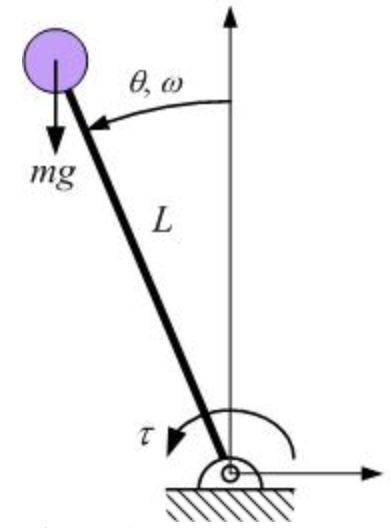
\includegraphics[width=2cm,height=3cm]{Figs/inv_pend.png}&	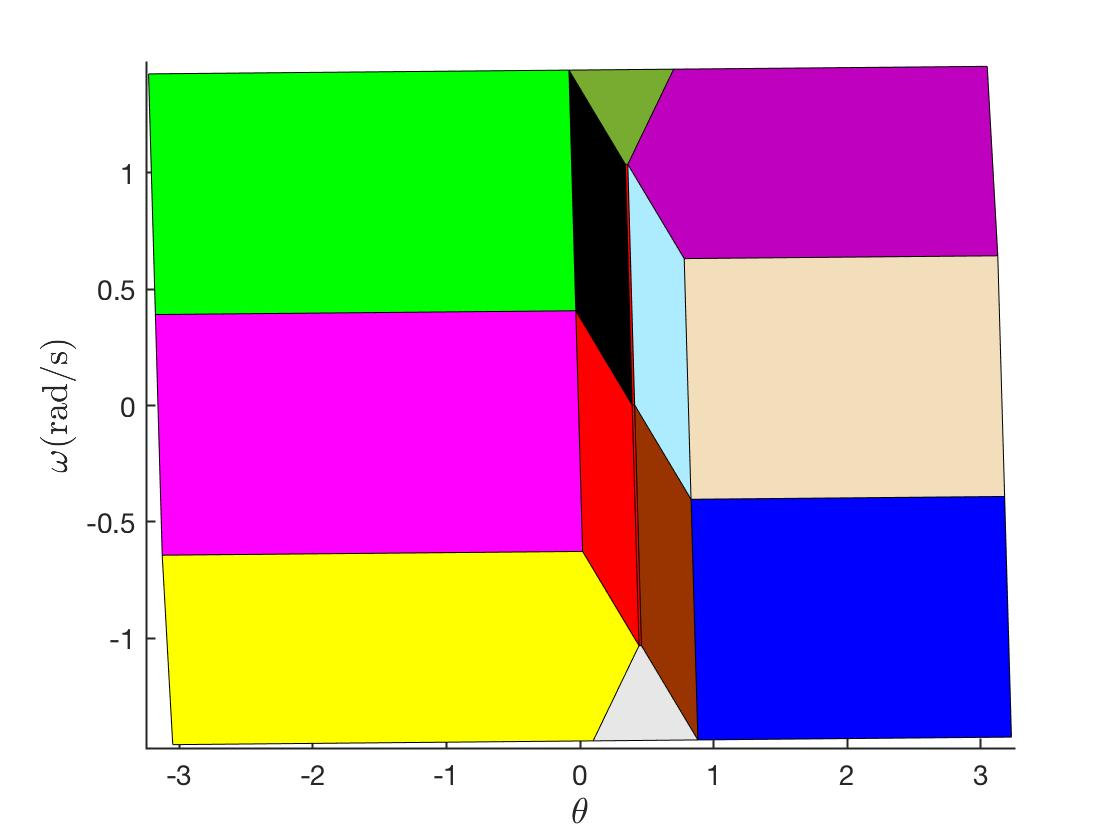
\includegraphics[width=6cm,height=4cm]{Figs/regs.jpg}\\
	(a)&(b)
	\end{tabular}
	\caption{(a) Inverted pendulum; (b) 2-D plot of polyhedral partitions for an explicit MPC applied to the inverted pendulum.}
	\label{fig:inverted_pendulum}
\end{figure}

As a smaller example, consider the standard problem of designing a controller for an inverted pendulum depicted in~\autoref{fig:inverted_pendulum}~{(a)}.
The goal of the controller is to keep the pendulum at the vertical position while satisfying hard constraints on the state variables and control inputs.
A model of the system can be constructed using physical principles. 
After linearization and time discretization, the model is
	\begin{equation}
		\begin{bmatrix}
			 \theta_{k+1}\\
			\omega_{k+1}
		\end{bmatrix}=
		\begin{bmatrix}
			1 & T_s\\
			\frac{T_sg}{L}& (1-\frac{T_sb}{mL^2})		
		\end{bmatrix}
		\begin{bmatrix}
			\theta_k\\
			\omega_k
		\end{bmatrix}+
		\begin{bmatrix}
			0\\
			\frac{T_s}{mL^2}
		\end{bmatrix}u_k + w_k
		\label{eq:pendul_ss}
	\end{equation}
where $\theta_k$, $\omega_k$, and $u_k$ denote respectively the angular position, angular speed, 
and the input torque at time $kT_s$ with $T_s$ being an appropriate sample time.
The disturbance $w_k\in\mathbb R^2$, bounded by $\|w_k\|\leq \Delta$, captures the modeling error due to 
linearization and discretization. 
The parameter $g=9.81 [m/s^2]$ is the gravitational acceleration, $m$ is the ball mass, $b$ is the rotational fraction coefficient, 
and $L$ is the length of the bar. 
Starting from an initial state $(\theta_0,\omega_0)$, the control goal is to converge to the equilibrium point 
$\theta=0, \omega=0$.
Additionally, we require the state constraints $\theta_k\in[-\pi,\pi]$ and $\omega_k\in[-\pi/8,\pi/8]$ to hold at all time instances.

Our overall goal is to 
(i) design a robust MPC controller that achieves the performance objectives including hard constraints in spite of a bounded
disturbance $\Delta$ modeling the implementation error due to finite precision;
and at the same time
\eva{what about the modelling error that $\Delta$ bounded in the paragraph before?}
(ii) to minimize the total number of bits that are required for storing the explicit controller 
while ensuring the error $e\leq \Delta$ is satisfied by the implementation.

% There are many control schemes that can guarantee convergence of the trajectories to the rest position (e.g., state feedback or linear quadratic regulator), but fail to ensure hard constraints on the states at all time instances. The main feature of MPC schemes is to automatically include these constraints in the design of control actions.
%	One major challenge of implementing model predictive controllers over embedded systems is to solve the related optimization within each sampled time inerval. Since the system under consideration is LTI, one can use explicit MPC \cite{Bemporad:2002} that computes partitions over state space together with affine functions which are then used to compute the optimal control input over their corresponding partition. For the inverted-pendulum example, the computed controller contains $12$ partition presented in Fig.~\ref{fig:inverted_pendulum}~{(b)}, each with an affine function that gives the control action over that partition.
	
%	In many practical applications, explicit MPC is implemented over relatively low-price embedded systems with limited memory capacity and computational power. The partitions together with the affine functions should be stored on the embedded system.
%	Computing the control action, i.e., evaluating the affine function for a specific state, can be performed efficiently using for example binary tree search. However, the memory limitations is more crucial since the memory usage increases linearly with the number of partitions.
%	In this paper we discuss a method for reducing the memory usage in applying explicit MPC to LTI dynamical systems.
	
%	Many low-end embedded systems only support fixed point arithmetic which causes errors that is inversely proportional to the number of bits used for representing each variable. It is necessary to account for such errors in the design stage of the controllers to be able to enforce hard constraints on the states at the final implementation of the controller. Our proposed method iteratively solves a robust version of the MPC with varying bound on the disturbance to include such errors.   %Therefore, one needs to formulate the problem as robust EMPC to count for disturbance input $|\delta|\leq \Delta$ which is summed up with the control input torque $u$ in each time step.
	 %Setting the number of bits for storing different variables, one can compute the upper bound for approximation error, $\bar\omega$.
	%However, we would like to achieve the minimum number of bits to reduce memory requirements.
	
%	In summary, we design a robust explicit MPC, taking fixed-point arithmetic errors into account and find a minimal set of mixed precision assignments for all the quantities that must be stored on the embedded system. 
% Denote the overall error produced by the fixed finite precision implementation by $e$.

%Our approach iteratively expand the bound on disturbance $\Delta+\Delta_0$, designs a robust explicit MPC controller with this bound and 
% uses state-of-the-art fixed-point error analyzers to find the minimum total number of bits for storing the controller into the embedded system with maximum error $\Delta_0$.
	
Figure \ref{fig:overview} gives a high-level overview of our proposed setup. 
We start by defining an initial bound $\Delta_0$. 
For our example, we choose $\Delta_0=0$. 
We use MATLAB to find a robust explicit MPC with the bound $\Delta_0$ on the disturbance.
Next, we ask Daisy
to provide us with a mixed-precision scheme such that the implementation satisfies the error bound $\Delta$, that is,
at all points in the control domain, the difference between the (infinite precision) controller function
and its implementation in the mixed-precision scheme is at most $\Delta$.

Unfortunately, $\Delta_0=0$ is not realizable,  as the error resulting from a fixed-point 
implementation is always greater than zero.
\eva{Is this the error due to mixed-precision or due to wrong regions?}
Therefore, we increase $\Delta$ by $0.05$ and try again. 
Solving the robust explicit MPC problem for the new disturbance bound gives the new controller,
shown in Figure~\ref{fig:inverted_pendulum}(b).
The controller has \RM{XX} regions.
\RM{give the control function. I think it will be good to explicitly write the polyhedra and the affine maps} 

Next, we ask Daisy to provide us with mixed-precision implementation for all the parameters and to compute a static bound on the
implementation error. 
The mixed-precision scheme given by Daisy results in an implementation with $6084$ bits in total 
for the corresponding robust explicit MPC.
Daisy also computes a static error bound of \RM{what?}
Since this error bound is less than our robustness margin $\Delta = 0.05$, we terminate the loop
and return this implementation.
The mixed-precision implementation takes about $10\%$ less memory compared 
to the smallest uniform precision implementation that respects $\Delta$,
and about $XXX\%$ \RM{what} less memory than an implementation that uniformly uses
32 bits.
	
	
	\tikzstyle{block} = [draw, rectangle, 
	minimum height=3em, minimum width=6em]
	\tikzstyle{sum} = [draw,  circle, node distance=1cm]
	\tikzstyle{input} = [coordinate]
	\tikzstyle{output} = [coordinate]
	\tikzstyle{pinstyle} = [pin edge={to-,thin,black}]
	\begin{figure*}[t]
		\begin{tikzpicture}[auto, node distance=2cm,>=latex',scale=1]
			\centering
			\node [block,scale=1,,text width=3.5cm, pin={[pinstyle]above:$\Delta=\Delta_0$},
			node distance=1cm] (RMPC) {Robust explicit MPC design (computed by MATLAB)};
			%\node[] (partitions) at (2.5,.5){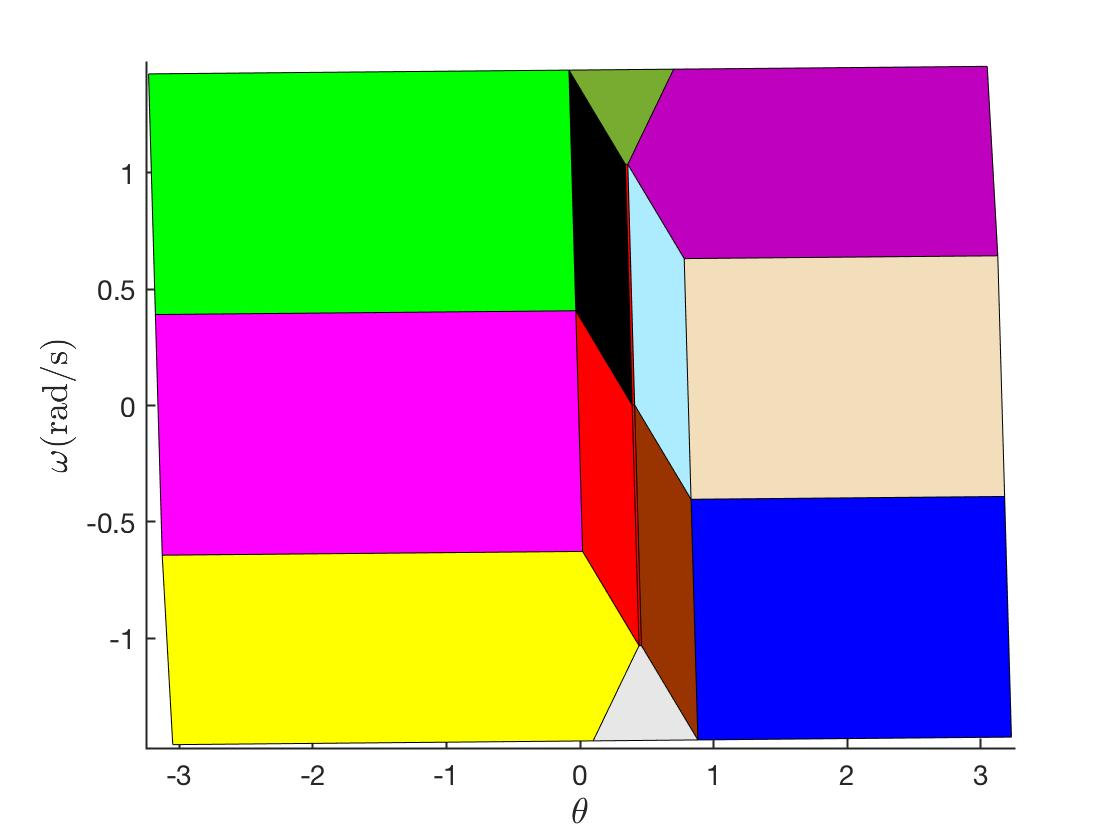
\includegraphics[width=.08\textwidth]{Figs/regs.jpg}};
			\node [block, scale=1,right=2.5cm of RMPC,
			node distance=5cm,text width=4cm] (mixed) {Finite precision implementation (computed by Daisy)};
			\node [draw, diamond, 
			minimum height=3em, minimum width=3em, right =1cm of mixed,
			node distance=5cm] (decide) {$e\leq \bar \Delta$};
			\node [block, right of=decide,
			node distance=3cm] (done) {Done};
			\node [block, below of= decide,
			node distance=3cm] (delta) {increase $\Delta$};
			\node [scale=1] at (3,-.25)  {
				$u(x)=Kx+v$
			};
		\node at (9,-.25) {$e$};
			
			
			\draw [draw,->] (RMPC) -- node [pos=-.1] {}(mixed);
			\draw [->] (mixed) -- node [name=aaa] {}(decide);
			\draw [->] (decide) -- node [above,pos=.3] {Yes} (done);
			\draw [->] (decide) -- node[pos=0.99] {} 
			node [] {No} (delta);
			\draw [->] (delta) -| node [above] {} (RMPC);
	
	\end{tikzpicture}
	\caption{high-level description of the proposed memory-efficient robust MPC design
\RM{what is $\bar{\Delta}$}
\RM{try to draw a better picture spanning only one column. the information in this pic is sparse}
\RM{why is $u$ a single affine map?}
\RM{why is Daisy only giving $e$? Shouldn't it also return the best mixed precision impl?}
}
	\label{fig:overview}
\end{figure*}

	

% !TEX root = main.tex
\section{Background}
In this section, we provide relevant background on robust explicit MPC,
fixed-point arithmetic and error analysis.

\subsection{Robust Explicit MPC}
\def\reals{\mathbb{R}}
We consider the class of linear time-invariant (LTI) systems characterized by the difference equation
\begin{equation}
\label{eq:DSS}
x_{k+1}=Ax_k+Bu_k+Ew_k,\quad  k=0,1,2,\ldots
\end{equation}
where $x\in \reals^{n\times 1}$ is the state, $u\in \reals^{m\times 1}$ is the control input and $w\in \reals^{d\times 1}$ is the disturbance. Matrices $A\in \reals^{n\times n}$, $B\in \reals^{n\times m}$ and $E\in \reals^{n\times d}$  capture respectively the effects of current state, input and disturbance on the next state. We assume the disturbance $w$ belongs to a set $\mathcal{W}$ where $\mathcal{W}$ is a polyhedral set.
In this paper, we focus on the robust formulation of MPC which at each time step
minimizes the worst-case value of an objective function with respect to the
disturbances over the control inputs. We assume the objective function is
quadratic with respect to the states and inputs.
We assume a linear translation on the input with the form
$$u_k=\mu x_k+v_k$$
and synthesize $v_k$ instead of $u_k$. This choice reduces the 
conservativeness of the optimization and enlarges the set of feasible input
trajectories. The matrix $\mu$ is selected such that some desired property is satisfied under suitable assumptions on the system, e.g., stability if the pair $(A,B)$ is stabilizable.

%\eva{I don't understand the above sentence. Maybe split into several sentences? Where does $u_k$ come from (the sentence right now says you assume $u_k$)?}
%The modifed state evolution of the system will be $x_{k+1}=\bar Ax_k+Bv_k+Ew_k$ with $\bar A := A +BK$.
% and $v_k=\kappa(x_k)$ denotes the output of model predictive controller.  
The constrained optimization at each time step is of the form
\begin{align}
\label{eq:RMPC_prob}
J^{\ast}(x_0)=&\min_{v_0,\cdots,v_{N-1}} \max_{w_0,\cdots,w_{N-1}} \sum_{i=0}^{N-1}(x_i^TQx_i+u_i^TRu_i) + x_N^TQ_Fx_N\nonumber\\
\text{s.t.} \quad &x_{i+1}=Ax_i+Bu_i + E w_i, \quad\forall i\in\{0,1,\cdots,N-1\}\nonumber\\
\quad &u_i=\mu x_i+v_i, \quad\forall i\in\{0,1,\cdots,N-1\}\nonumber\\
&u_i\in\mathcal{U},x_i\in\mathcal{X},\quad \forall w_i\in\mathcal{W},\,\,\forall i\in\{0,1,\cdots,N\},
%&x_i\in\mathcal{X},\quad \forall w_i\in\mathcal{W},\quad\forall i\in\{0,1,\cdots,N\},
\end{align}
%\Sadegh{The role of disturbance is missing in the inequalities. We should say, we want to satisfy the inequalities for all possible values of the disturbance.}
%
where $\mathcal U$ and $\mathcal X$ are polyhedral sets denoting the feasible
sets of inputs and states. Positive definite matrices $Q\in\reals^{n\times n}$ and
$Q_F\in\reals^{n\times n}$ indicate weights on the states. $R\in\reals^{m\times m}$ is
positive semidefinite and indicates a weight on the input in the objective function. $N$ denotes the length of the prediction horizon.
%\eva{What are $Q, Q_F, R$ and where do they come from?}

\begin{theorem}[\cite{delaPea:2005}]
\label{thm:EMPC}
The optimization \eqref{eq:RMPC_prob} can be translated into a multi-parametric quadratic problem which admits a closed-form solution. Furthermore, for the case that $R>0$, the controller is $u_k = \mu x_k + \kappa(x_k)$ with $\kappa(\cdot)$ being a continuous piecewise affine (PWA) function over polyhedral regions:
\begin{equation}
\label{eq:affine_map}
\kappa(x_k)=
\begin{cases}
F_1x_k+G_1 & \text{if $x_k\in \mathcal{R}_1$}\\
F_2x_k+G_2 & \text{if $x_k\in \mathcal{R}_2$}\\
\vdots\\
F_Px_k+G_P & \text{if $x_k\in \mathcal{R}_P$}
\end{cases} 
\end{equation}
where $\mathcal{R}_i$ is a polyhedral region determined by a set of linear inequalities $\mathcal R_i = \{x\in\mathcal X\,|\,H_ix\leq K_i\}$. 
\end{theorem}
The essential idea behind this theorem is to utilize the closed form $x_i=A^ix_0+\sum_{l=0}^{i-1}A^{i-l-1}Bu_l$ and transform the optimization \eqref{eq:RMPC_prob} into the following quadratic program:
%\begin{align}
%	&\min_{U_N}U_N^TZU_N+x_0^TVU_N+x_0^TYx_0\nonumber\\
%	&s.t.\quad JU_N\leq s+Dx_0
%\end{align} 
\begin{align}
\label{eq:multi_param_prog}
J^{\ast}(x_0)=\min_{z,\gamma}& \left[x_0^TYx_0+\frac{1}{2}z^THz+\gamma\right]\\
\text{s.t.} \quad &G_mz+g_m\gamma\leq W_m+S_mx_0,\nonumber\\
&G_cz\leq W_c+S_cx_0\nonumber
\end{align}
where $z\in \reals^{mN}$ and $\gamma\in\reals$ are decision variables, and $Y$, $H$, $G_m$, $G_c$, $S_m$, $S_c$, $W_m$, $W_c$, and $g_m$ 
are matrices of proper sizes that can be easily obtained from the original optimization \eqref{eq:RMPC_prob}  (see \cite{delaPea:2005}).

%\Sadegh{Adding a remark and saying that the approach works as long as the solution of formulated optimization has a piecewise affine form?} 

The optimization \eqref{eq:multi_param_prog} can be solved using multi-parametric techniques to compute the explicit form of $\kappa(\cdot)$.
An efficient implementation of such computations is available in the multi-parametric toolbox of Matlab~\cite{matlabMPT, matlabYALMIP}.
Let us denote the set of states $x_0$ for which the optimization  \eqref{eq:multi_param_prog} is feasible by $\mathcal X_s$. Then $\mathcal X_s\subseteq \mathcal X$ and is the union of all regions $\mathcal{R}_{i}$:
\begin{equation}
\mathcal X_s = \bigcup_{i}(H_{i}\statevar\leq K_{i}).
\end{equation}


The implementation of the controller stores the matrices $F_i,G_i,H_i,K_i$ for all $i\in\{1,2,\ldots,P\}$. 
At each time step $k$, the current state $x_k$ is used to detect the polyhedral region 
such that $H_i x_k\le K_i$. Then the control action $v_k = F_i x_k + G_i$ is computed and applied to the system.
Several algorithms are proposed in the literature \cite{Mnnigmann:2011,Jones:2006} to find the right polyhedral region $i$ to which the state $x_k$ belong. 
The most straightforward technique is a linear search over all polyhedral regions (Fig.~\ref{lst:caseof}).

\begin{figure}[t]
\begin{lstlisting}[mathescape=true,basicstyle=\small\ttfamily,morekeywords={if, then, elseif, return}]
if ($H_{1}\statevar \leq K_{1}$) then $v_{k}=F_1x_k+G_1$
elseif ($H_{2}\statevar \leq K_{2}$) then $v_{k}=F_2x_k+G_2$
elseif ($H_{3}\statevar \leq K_{3}$) then $v_{k}=F_3x_k+G_3$
...
elseif ($ H_{P}\statevar\leq K_{P}$) then $v_{k}=F_Px_k+G_P$
return $v_k$
\end{lstlisting}
\caption{Structure of an explicit MPC controller}
\label{lst:caseof}
\end{figure}
%Once the polytope was determined, computing for $F_ix+G_i$ requires even less effort as it only involves summation and multiplication.  

To keep the implementation cost down, low-end microcontrollers usually have
limited memory and computational power. Therefore, the implementation of the above
explicit MPC on microcontrollers will bring some issues since all regions'
matrices ($H_i$s and $K_i$s) and activation functions ($F_i$s and $G_i$s) have
to be stored on the microcontroller. Our paper presents an
approach for minimizing the memory usage of the implementation while satisfying
the hard constraints on the states.
%\section{Finite Precision Implementation}
%\Sadegh{To be included by Rocco}

%!TEX root = main.tex
\subsection{Finite-Precision Implementation}

The controller has to be stored and evaluated on a microcontroller in
finite precision, since infinite-precision real values cannot be stored on
today's digital computers.
The standard choice for low-power platforms is fixed-point arithmetic. Unlike
floating-point arithmetic~\cite{ieee75408}, fixed-point arithmetic can be implemented efficiently
without complex hardware support using only integer operations. It requires,
however, more compilation effort to determine certain operations statically at
compile time (that the floating-point hardware unit performs dynamically).
 
% general blob about fixed-point arithmetic
The main task at compile time is to select the fixed-point format for each input and intermediate value
in the program. The format specifies the total word length and how many bits are
available for the integer part of the number. Given ranges on program inputs, a
range analysis is usually used to estimate ranges of all intermediate values in the
program~\cite{Pang2011,Kinsman2009}, which in turn determine how many integer bits are sufficient to
avoid overflow. The remaining bits of the total word length represent the
fractional part of a number; more fractional bits provide more precision. 

% introduces roundoff errors, these can be tracked with a dataflow analysis
Finite precision unavoidably introduces roundoff errors, which can accumulate
during the course of a computation.
A sound static roundoff error analysis computes a guaranteed upper bound on the
error of the result by tracking worst-case errors at every operation. Given a
word length for each value, several tools\Eva{, including the tool Daisy which we use,} automatically determine the number of
integer bits needed and compute roundoff errors using a dataflow analysis~\cite{Daisy,Gappa}.
They track real-valued ranges at every intermediate operation. These ranges
determine the fixed-point formats and thus also the individual worst-case roundoff errors,
which the analyses track separately from the ranges. To ensure guaranteed
error bounds, both the ranges and errors are computed using interval~\cite{intervals} or
affine arithmetic~\cite{affineArithmetic} which compute sound enclosures. 
Affine arithmetic tracks linear correlations between variables, so for linear expressions
the computed ranges are as tight as possible (nonlinear arithmetic
leads to over-approximations).
% A standard technique to increase accuracy of the computed errors is interval
% subdivision, which divides the input domain into equally-sized subdomains and
% runs roundoff error analysis separately for each subdomain. The
% over-approximations on each subdomain tend to be smaller, which increases the
% overall tightness of range and error bounds.

% mixed-precision tuning
To reduce memory usage and increase efficiency, we want to choose as short word
lengths as possible, \Mahmoud{as this way memory footprint is minimized and run-time is not influenced.} Mixed-precision tuning tools automatically determine possibly different
word lengths for different values~\cite{DaisyTuning,Lee2006}. Compared to uniform precision (or word length),
mixed-precision often leads to improved resource usage, but due to the complexity of
fixed-point arithmetic and the error analysis, is challenging to do manually.  
Automated mixed-precision tuning tools\Eva{, including Daisy,} usually perform a search: they repeatedly
select a candidate mixed-precision assignment (i.e. different word lengths for
different values) and check whether the assignment satisfies a given error
bound. The candidate assignments are chosen based on a heuristic which guides
the search towards promising candidates, e.g. using delta-debugging~\cite{DaisyTuning} or
simulated annealing~\cite{Lee2006}.

In this work, we use the tool Daisy which implements roundoff error
analysis~\cite{Daisy} and mixed-precision tuning~\cite{DaisyTuning} for fixed-point arithmetic, and is
available as open-source. Fixed-point arithmetic implementations can choose different
rounding modes; here we consider truncation, which is more efficient than
rounding.%temporary
%!TEX root = main.tex
\section{Error Analysis}
\label{sec:Error_Analysis}

In this section, we present our error analysis assuming that a fixed word length $p$ is given.
Then in the next section, we explain our optimization algorithm which determines suitable word
lengths for different variables fully automatically. % in~\autoref{sec:Controller_Synthesis}.
%
% For simplicity of notation, we assume in this section a uniform word length $p$,
% but our algorithm (and implementation) is applied to mixed-precision to reduce the memory usage.

Consider the controller obtained from explicit MPC according to Theorem~\ref{thm:EMPC}.
Define the affine control functions associated with each polyhedral region $\mathcal R_i$, $i\in\{1,2,\ldots, P\}$, as
$$v_{i}:\mathcal R_i\rightarrow \mathcal U \quad \text{ with } \quad v_{i}(x) := F_i x + G_i.$$
Implementation of the controller can be affected by two main sources of
error:
%which an error analysis has to capture \cite{imperialrmpc}:
\begin{itemize}
  \item[(i)] \emph{incorrect region selection}:
   instead of a correct affine function $v_{i}$, the implementation may choose an incorrect affine function $v_{j}$. This can happen either
    due to an analog-to-digital conversion in the measured states or due to the quantization in matrices $H_i$ and $K_i$ of the region $\mathcal R_i$; and
    
  \item[(ii)] \emph{approximation in the computation of the affine function}: for any selected region $\mathcal R_i$, the affine function $v_{i}$ is evaluated using the quantized versions of $F_i$ and $G_i$.
\end{itemize}

We have to ensure that the sum of these two errors remain below the bound $\Delta$
used in the design of the robust explicit MPC:
\begin{align}
  \max\{\|v_{i}-v_{j}\|,\,&\forall i,j,\,\, i\neq j, \mathcal{R}_{i}\cap\mathcal{R}_{j}\neq\emptyset\} \nonumber\\
  &+  \max\{err(v_{i})_{p},\, i=1,2,\ldots,P\} \le \Delta.
  \label{eq:delta}
\end{align}
%where $i,j$ are the indexes of two distinct regions $\mathcal{R}_{i}$ and $\mathcal{R}_{j}$, 
The first term is the error of incorrect region selection. The maximum is taken over all neighboring regions 
$\mathcal R_i,\mathcal R_j$ (two regions are neighboring if their intersection is non-empty).
The function norm $\|v_{i}-v_{j}\|$ is taken by maximizing over all possible values of the state $x_k$. 
$err(v_{i})_{p}$ in
the second term captures the approximation error in the computation of the affine function $v_{i}$ when a fixed precision $p$ is used.
%$\mathit{neighbor}(\mathcal{R}_{i},\mathcal{R}_{j})$
%states that two regions share at least a point, $v_{i}$ is the control action
%for controller $i$, and $err(v_{i})_{p}$ captures the approximation error for
%computing the control action $v_{i}$ in fixed precision $p$.

\subsection{Incorrect Region Selection}

The first part of the error in~\autoref{eq:delta} captures the error due to
selecting of the incorrect region.
This would happen since the matrices $H_i,K_i$ are stored in the hardware with fixed-point formats. In order to quantify the error, we define the expanded border $\bar{\mathcal B}_{ij}$ as the tube around the border between the regions $\mathcal{R}_i$ and $\mathcal{R}_j$:
% \begin{equation*}
% \bar{\mathcal R}_i := \bigcup_{\hat H_i,\hat K_i} \left\{x\in\mathbb R^n\,|\,\hat H_i x\le \hat K_i, \|H_i-\hat H_i\|\le \epsilon_f,\|K_i-\hat K_i\|\le \epsilon_f\right\}
% \end{equation*}
% for $i\in\{1,2,\ldots, P\}$, where $\epsilon_f$ is the maximum error of using fixed-point format instead of the precise values. The norm is also applied element-wise to the entries of the matrices. 

\begin{equation*}
\hat{\mathcal B}_{ij} := \left\{x\in\mathbb R^n\,|\, \| H_i x - K_i\| \le \varepsilon\,\, \text{ and }\,\, \| H_j x - K_j\| \le \varepsilon \right\},
\end{equation*}
where $\varepsilon$ captures the uncertainty in computing the correct region.
%
The width of the tube $\varepsilon$ is due to two sources of errors:
analog-to-digital conversion $\varepsilon_{A/D}$ and the quantization of region
bounds in memory $\varepsilon_{Q}$:
\begin{equation}\label{eq:epsilontot}
  \varepsilon=\varepsilon_{A/D}+\varepsilon_{Q}
\end{equation}

Analog conversion happens just before the controller receives the sensor input from the plant
and is given by:
\begin{equation*}
\varepsilon_{A/D}=\frac{V_{cc}}{2^{r}-1}
\end{equation*}
where $V_{cc}$ is the reference voltage of the converter (e.g. typically 5V), $r$
is the number of bits available to quantize the analog signal, and $2^{r}$ is
the resolution of the converter.

While $\varepsilon_{A/D}$ is intrinsic to the capabilities of the device,
$\varepsilon_{Q}$ depends on the precision used to store the boundaries:
\begin{equation}\label{eq:quantizationlines}
  \varepsilon_{Q} \ge  \|(H_i - \hat{H}_i) \hat{x} + (K_i - \hat{K}_i)\|, \quad \forall \hat{x},\forall i,
\end{equation}
where $\hat{x}$ is the finite-precision value of $x$.
%\eva{For which index is this evaluated, $i$, $j$ or both?}
That is, $\varepsilon_{Q}$ bounds the distance between any hyperplane in infinite
precision ($H$ and $K$ matrices), and its counter-part quantized by $p$ bits 
($\hat{H}_{p}$ and $\hat{K}_{p}$).
This second error can be tuned providing a trade-off between accuracy and
memory storage required.

% Note that $\mathcal R_i\subset \bar{\mathcal R}_i$. In other words, $\bar{\mathcal R}_i$ is the expanded version of $\mathcal R_i$.
% Note that $\bar{\mathcal R}_i\cap \bar{\mathcal R}_j$ gives us the states where one of the two regions $\mathcal R_i, \mathcal R_i$ might be selected instead of the other one because of the fixed-precision implementation of the regions.   
% $\bar{\mathcal R}_i$ is the expanded version of $\mathcal R_i$ that include all states in $\mathcal R_i$this definition expands the regions $\mathcal $
 %That is, with infinite-precision arithmetic
 Therefore, the first term in~\autoref{eq:delta} can be computed less conservatively by maximizing only over 
 the expanded borders:
 \begin{equation}
 \label{eq:maximization}
 \max_{x,i,j}\{\|F_ix+G_i-F_jx-G_j\|,\,x\in \bar{\mathcal B}_{ij}\}.
% \max_{\forall i,j.\mathit{neighbor}(\mathcal{R}_{i},\mathcal{R}_{j})}&|F_{i}\statevar+G_{i} - (F_{j}\statevar+G_{j})|
 \end{equation} 
 
%and in the absence of any uncertainty from hardware measurements we would choose
%control action $v_{i}$, but due to uncertainties we actually choose control action $v_{j}$:
%\begin{align} \label{eq:maximization}
 % \max_{\forall i,j.\mathit{neighbor}(\mathcal{R}_{i},\mathcal{R}_{j})}|v_{i}-v_{j}|&= \\
 % \max_{\forall i,j.\mathit{neighbor}(\mathcal{R}_{i},\mathcal{R}_{j})}&|F_{i}\statevar+G_{i} - (F_{j}\statevar+G_{j})|\nonumber
%\end{align}

%Because of the linearity of the function $v_{i}-v_{j}$, and because of the
%convexity of the regions $i$ and $j$, it is enough to evaluate function
%(\ref{eq:maximization}) at the corner points of the \texttt{tube}, instead of
%solving a maximization problem.

%A naive computation of this error would consider all possible values of $x_k$.
%This would lead to a gross over-approximation, however, since the controller
%will choose a wrong region only in a relative narrow neighborhood, or
%\emph{tube}, around the boundary between two regions $R_i$ and $R_j$.

%The border between two regions $\mathcal{R}_{i}$ and $\mathcal{R}_{j}$ is defined by 
%their corresponding boundaries:
%\begin{equation}
%\mathit{border}_{i,j} :=(H_i \statevar - K_i ) - (H_j \statevar - K_j)
%\end{equation}
%for appropriate matching borders $H_i, K_i$ and $H_j, K_j$.

%In~\autoref{eq:maximization}, we thus constrain $\statevar$ to be within an appropriate tube:
%\begin{equation}\label{eq:tube}
%|\mathit{border}_{i,j}| \le \varepsilon
%\end{equation}
%where $\varepsilon$ captures the uncertainty in computing the
%correct region and thus the width of the tube.
%

\begin{comment}
We should also include the error in 
The width of the tube $\varepsilon$ is due to two sources of errors:
analog-to-digital conversion $\varepsilon_{A/D}$ and the quantization of region
bounds in memory $\varepsilon_{Q}$:
\begin{equation}\label{eq:epsilontot}
  \varepsilon=\varepsilon_{A/D}+\varepsilon_{Q}
\end{equation}

Analog conversion happens just before the controller receives the sensor input from the plant
and is given by:
\begin{equation*}
\varepsilon_{A/D}=\frac{V_{cc}}{2^{r}-1}
\end{equation*}
where $V_{cc}$ is the reference voltage of the converter (e.g. typically 5V), $r$
is the number of bits available to quantize the analog signal, and $2^{r}$ is
the resolution of the converter.

While $\varepsilon_{A/D}$ is intrinsic to the capabilities of the device,
$\varepsilon_{Q}$ depends on the precision used to store the boundaries:
\begin{equation}\label{eq:quantizationlines}
  \varepsilon_{Q} \ge  |(H_i - \hat{H}_i) \qstatevar + (K_i - \hat{K}_i)|, \forall  \qstatevar
\end{equation}
\eva{For which index is this evaluated, $i$, $j$ or both?}
That is, $\varepsilon_{Q}$ bounds the distance between any hyperplane in infinite
precision (H and K), and its counter-part quantized in $p$ bits precision
($\hat{H}_{p}$ and $\hat{K}_{p}$).
This second error can be tuned providing a trade-off between accuracy and
memory storage required.
\end{comment}


\subsection{Approximate Control Output}

% We should also include the error due to
% analog-to-digital conversion $\varepsilon_{A/D}$.
% Analog to digital conversion happens just before the controller receives the measured state from sensor
% and is given by:
% \begin{equation*}
% \varepsilon_{A/D}=\frac{V_{cc}}{2^{r}-1}
% \end{equation*}
% where $V_{cc}$ is the reference voltage of the converter (e.g. typically 5V), $r$
% is the number of bits available to quantize the analog signal, and $2^{r}$ is
% the resolution of the converter. The associated error in the output of the controller is $\varepsilon_{A/D}\max_i\{\|K+F_i\|\}$.

Once a quantized state $\hat x$ is given and a region $\mathcal R_i$ is chosen, computing $v_{i}$ itself introduces
imprecision, because, $v_{i}$ needs to be evaluated in finite-precision arithmetic:
\begin{equation}\label{eq:fperror}
  err(v_{i})_{p} \ge  | (F_i - \hat{F}_{i}) \statevar + ( G_i - \hat{G}_{i} ) |,\quad \forall \statevar\in \mathcal{R}_i\cup\bar{\mathcal B}_{ij},\,\,\forall j,
\end{equation}
where $\hat{F}$ and $\hat{G}$ represent the quantized values (in $p$ bits) for
the infinite precision values $F$ and $G$.

\autoref{eq:fperror} is evaluated for all \statevarmath that are inside the
region $\mathcal{R}_i$, together with all the values in the tube surrounding
region $\mathcal{R}_i$ (union of $\bar{\mathcal B}_{ij}$ for all $j$).
In this way we compute the error also for those points that belong to a neighbor
of $\mathcal{R}_i$, but because of finite-precision errors they are erroneously
mapped to control action $v_{i}$.

\subsection{Implementation}

The incorrect region error (\autoref{eq:maximization}) is computed with Matlab. 

Since $v_{i}-v_{j}$ is also affine, and because we defined the tube as a convex region 
surrounding the corresponding hyperplane, it suffices
to evaluate the function only at the corner points of the tube, and keep the
result with the maximal magnitude. 
To evaluate the incorrect region selection error across
the corner points, we need to first locate the corner points as well as all the
regions which share those corner points. 
Each region $R_i$ is represented by a set of contraints. We first extract the
set of vertices of $R_i$ using the open source Matlab library
$\mathit{lcon2vert}$~\cite{lcon2vertMatlab}.
For each computed vertex $v_i$, we compute a $n$-dimensional
hypercube with the edge length of $2 \varepsilon$. 
Each of the $2^n$ vertices of this hypercube is counted as a corner point, on which
we evaluate $\|u_i - u_j\|$. 

In order to find out which regions share a vertex $v_i$, we implemented two approaches.
The first approach determines the set of neighboring regions via an exhaustive
search over the set of vertices. However, we observed that this algorithm only
scales to small numbers of regions.
Our second approach works on the observation that all the regions $R_j$s 
having $v_i$ as their vertex can be identified if at least $n$ of their hyperplanes cross $v_i$. 

% In brief, we go
% through these steps: (i) for each region, the set of vertices are computed; (ii)
% for the vertex $v_i$, the set of all regions $\mathcal R_{ij}$ having $v_i$ as
% their own vertex are found; (iii) for the vertex $v_i$, the set of corner points
% $v_{ik}$ are computed which form a hypercube centering at $v_i$; (iv) for every
% corner point $c_k=v_{ik}$ and for every pair $(\mathcal R_{ij1},\mathcal
% R_{ij_2})$, the corresponding corner error $|v_{j1}-v_{j2}|$ is computed; (v)
% finally, we pick the greatest corner error.

% \eva{This needs more details. Which function(s) and algorithm from Matlab are used?}
% \eva{How do you determine which regions are neighbors? resp. which borders are matching?}

The error terms $\varepsilon_Q$ and $err(v_{i})_{p}$ are computed by Daisy. For this we encode
the expressions in~\autoref{eq:quantizationlines} and \autoref{eq:fperror}
respectively as straight-line arithmetic expressions and specify the constraints
on the domain of $\statevar$ in the precondition.
Daisy performs a dataflow analysis to determine the finite-precision roundoff
errors. 
% This error computation differs from the one employed by
% \citet{imperialrmpc} which phrases the roundoff error computation as a (relaxed)
% mixed integer programming problem.

While our actual synthesis algorithm (\autoref{sec:Controller_Synthesis}) does
not compute the errors $\varepsilon_Q$ and $err(v_{i})_{p}$ explicitly, the
error verification is used internally by Daisy to determine a suitable precision
$p$ and can also be called explicitly without the precision optimization.

\begin{comment}
\textcolor{red}{Sadegh: This is long comment on the content of this section. I cannot figure out how this line of reasoning is mapped to the implementation. We can discard my comment given that we are close to the deadline.}

\Sadegh{
I don't agree that we should add $\varepsilon_{A/D}$ and $\varepsilon_Q$ together. I understand that the implementation is done according to this, but I think we need to multiply $\varepsilon_{A/D}$ by the maximum norm of the coefficients $F_i$ in the controller. There are three approximations:
\begin{itemize}
\item using the quantized measured state $\hat x$ instead of the actual state $x$. We assume $\|x - \hat x\|\le \varepsilon_{A/D}$.
\item using $\hat H_i,\hat K_i$ which are the quantized versions of $H_i,K_i$ with $p$ bits precision. This is related to the boundaries of the regions.
\item using $\hat F_i,\hat G_i$ which are the quantized versions of $F_i,G_i$ with $p$ bits precision. This is related to the affine functions.
\end{itemize}
Let me define the sets $\mathcal H := \{H_i,K_i,i=1,2,\ldots, P\}$ and $\mathcal F:=\{F_i,G_i,i=1,2,\ldots, P\}$. Similarly, we define $\hat{\mathcal H}$ and $\hat{\mathcal F}$.
The controller (which is a piecewise affine function) can be written as the parametric function $\kappa(\mathcal H,\mathcal F,x)$. Our main goal is to make sure that
$$\|\kappa(\mathcal H,\mathcal F,x)-\kappa(\hat{\mathcal H},\hat{\mathcal F},\hat x)\|\le \Delta,\quad \forall x\in\mathcal X_{\mathsf s}.$$
We use tirangle these inequality:
\begin{align*}
\|\kappa(\mathcal H,\mathcal F,x)-\kappa(\hat{\mathcal H},\hat{\mathcal F},\hat x)
\|\le&\|\kappa(\mathcal H,\mathcal F,x)-\kappa(\hat{\mathcal H},\mathcal F,\hat x)\|\\
+&\|\kappa(\hat{\mathcal H},\mathcal F,\hat x)-\kappa(\hat{\mathcal H},\hat{\mathcal F},\hat x)\|.
\end{align*}
The second term is exactly what we have in section 4.2 (error in the evaluation of the affine function).
The first term can be further decomposed as
\begin{align*}
\|\kappa(\mathcal H,&\mathcal F,x)-\kappa(\hat{\mathcal H},\mathcal F,\hat x)\|\\
&\le \|\kappa(\mathcal H,\mathcal F,x)-\kappa(\mathcal H,\mathcal F,\hat x)\|+
 \|\kappa(\mathcal H,\mathcal F,\hat x) - \kappa(\hat{\mathcal H},\mathcal F,\hat x)\|\\
&\le \max_i\{\|F_i\|_2\}\|x-\hat x\| + \varepsilon_Q\\
& \le \max_i\{\|F_i\|_2\}\varepsilon_{A/D}+ \varepsilon_Q.
\end{align*}
The error $\varepsilon_{A/D}$ shows itself in the output of the controller by being amplified with the Lipschitz constant of the function which is $\max_i\{\|F_i\|_2\}$. 
As far as I can tell, $\varepsilon_{A/D}$ doesn't have anything to do with $\varepsilon_Q$. The computation of $\varepsilon_Q$ should be only with respect to the use of $\hat{\mathcal H}$ instead of $\mathcal H$ in the evaluation of constraints for the same value $\hat x$.
}
\end{comment}
% The approximation error and the precision tuning for both borders and active
% functions are computed in Daisy. $\varepsilon_{Q}$ is given in input to the
% analysis. After we compute the incorrect region in MATLAB we obtain the value
% for max error $err(v_{i})$ from (8). Then we give the errors and the vectors F,G
% and H,K in input to Daisy. We used Daisy as a verification tool: we provide in
% input the expression we want to quantize (e.g. $\mathcal{R}_{i}$) together with
% the error bound we can tolerate (e.g. $\varepsilon_{Q}$), and Daisy returns a
% precision configuration (uniform or mixed) such that the input error is
% satisfied. The way it finds the right configuration for uniform precision is the
% following: it starts by checking whether the input expression, quantized in
% unary uniform precision (1bit), introduces an error bounded by the input error.
% If this is not the case, Daisy increases the precision format by 1 bit and check
% whether the error now is satisfied. This unary increment runs inside a loop that
% terminates when the first valid format is matched. This uniform word-length is
% going to be the baseline for the mixed-precision tuning phase. The
% mixed-precision algorithm keeps a list of variables to quantize, and collects
% different candidate configurations that satisfy the input error. It returns the
% best configuration based on the evaluation of a quality function.



%!TEX root = main.tex
\section{Controller Synthesis}\label{sec:Controller_Synthesis}

\begin{figure}
\begin{lstlisting}[language=Python,numbers=left,numbersep=3pt,frame=lines,keepspaces=true,mathescape=true,basicstyle=\small\ttfamily,escapeinside={<@}{@>}]
 model = input() 
 $\Delta$ = input()
 $\varepsilon_{Q}$ = input()
 assert ($\Delta$ >= 0 and $\varepsilon_{Q}$ > 0)
 $\varepsilon$ = $\varepsilon_{A/D}$ + $\varepsilon_{Q}$<@\Mahmoud{//the width of the uncertain area}@>

 while true:
   $F$, $G$, $H$, $K$ = design_robust_MPC(model, $\Delta$)
   errorRegion = incorrect_region_error($F$, $G$, $H$, $K$, $\varepsilon$)
   if $\Delta$ > errorRegion:
     errorAct = $\Delta$ - errorRegion
     $\hat{F}$, $\hat{G}$ = precision_tuning($F$, $G$, errorAct)
     $\hat{H}$, $\hat{K}$ = precision_tuning($H$, $K$, $\varepsilon_Q$)
     return $\hat{F}$, $\hat{G}$, $\hat{H}$, $\hat{K}$
   else:
     $\Delta$ = errorRegion + $\varepsilon_{SAFE}$
\end{lstlisting}
\caption{Algorithm for designing memory-efficient robust EMPC controller}
\label{lst:alg}
\end{figure}

%\eva{The algorithm in \autoref{lst:alg} needs to be fixed:
%\begin{itemize}
  %\item Use the math symbol for Delta to be consistent with the rest of the paper
  %\item the function design\_robust\_MPC seems to do a lot more than just designing the controller, i.e. it seems to return an error bound instead of a controller. Split into more steps.
  %\item \maxUij and $err_{max}(u_{i})_{p}$ are not good variable names, use a proper variable name
  %$\item UNI\_MIX\_precision should also be renamed to something more helpful, e.g. tune\_precision?
%\end{itemize}
%}

In the previous section, we assumed a given precision $p$. In this section we
present our algorithm for deriving suitable values of $p$ fully automatically.
Further, while~\autoref{sec:Error_Analysis} assumed a uniform finite precision,
our tuning algorithm derives possibly different precisions for different control
values.

%\subsection{Algorithm}
\autoref{lst:alg} shows a high-level view of our optimization algorithm for
implementing robust MPC controllers with guaranteed error bounds.

Given a state-space model of a plant (line 1), our algorithm returns four matrices
$\hat{F}$, $\hat{G}$, $\hat{H}$, and $\hat{K}$,
which soundly implement a robust explicit MPC controller in mixed-precision
fixed-point arithmetic.
Our algorithm takes two additional inputs, $\Delta$ and $\varepsilon_Q$ (line 2, 3). 
The disturbance $\Delta$ provided by the user represents a starting point for 
the search for a robust controller. In principle, the user can set $\Delta = 0$,
however note that the finite-precision implementation of the controller will always
incur at least some small error. In practice we thus start the search with a slightly
larger value, e.g. $\Delta = 0.1$. Our algorithm will perform a linear search and
increase $\Delta$ if needed.

The third input parameter is $\varepsilon_Q$. In~\autoref{sec:Error_Analysis} we
showed that if the user provides a precision $p$, then we can automatically
compute $\varepsilon_Q$.
Now, we want to \emph{derive} a suitable precision $p$, however, and face an
issue. In order to derive $p$ for some expression, Daisy and any other precision
tuning tool requires an error bound which should be satisfied. I.e. either a
precision $p$ is given, and we can compute an error bound, or the error bound is
given and we can derive a precision $p$. We cannot do both at the same time; the
problem would be underconstrained. We solve this chicken-and-egg issue by
requiring the user to provide $\varepsilon_Q$ as the input. 
\Mahmoud{
	\begin{remark}\label{rem:eps_Q}
		Typical values for $\varepsilon_Q$ can range from $10^{-4}$ up-to $10^{-2}$. Increasing the $\varepsilon_Q$ leads into more memory save over $H$ and $K$, while requiring more precision for $F$ and $G$ (\autoref{tab:di}). Of course, too large values for $\varepsilon_Q$ can result in failure of RMPC design. However, this is usually not the case over reasonable choices for $\varepsilon_Q$.
	\end{remark}}

We need to distribute the available `disturbance budget' among the two error
sources: error due to selecting the wrong region, which is given by the
quantization of $\hat{H}$ and $\hat{K}$, and the error due to
quantization of the control action, given by $\hat{F}$, $\hat{G}$.
The quantization of $\hat{H}$ and $\hat{K}$ is determined by
$\varepsilon_Q$, thus by providing this input value, the user effectively
chooses how much precision to allow for $\hat{H}$ and $\hat{K}$.
Note that this precision comes at the expense of the precision of
$\hat{F}$ and $\hat{G}$, i.e. the more accurately $\hat{H}$
and $\hat{K}$ are represented, the more approximate $\hat{F}$ and
$\hat{G}$ need to be and vice versa.
We note that one could straight-forwardly extend our algorithm to include an
outer loop which would explore different values for $\varepsilon_Q$. For our
experiments in~\autoref{sec:experiments}, we vary this value manually.


% From line 1 to 3, the procedure waits for input parameters from the designer: $\delta$ and $\varepsilon_{Q}$. $\delta$ is the disturbance . It is a problem dependent parameter, and thus can be any positive number. Typically, it is in the order of 0.1.
% $\varepsilon_{Q}$ is the imprecision error-bound for the quantization of borders. 
% The latter has to be strictly greater than zero, otherwise we could rely on infinite precision for storage of borders. Usually, the value for $\varepsilon_{Q}$ is in the order of 0.001.

Unlike the initial $\Delta$, $\varepsilon_Q$ needs to be strictly positive (line 4)
for mixed-precision tuning tools to work correctly.
Line 5 computes the width of the tubes $\varepsilon$ as shown in~\autoref{eq:epsilontot},
which will be used to bound the error due to selecting the wrong region
($\varepsilon_{A/D}$ is a constant parameter dependent on the specifics of the
converter).

The algorithm then calls Matlab's multi-parametric toolbox to design an explicit
MPC controller for the given state-space model which is robust to the initial
disturbance $\Delta$ (line 8). The result is a controller represented by four matrices
$F$, $G$, $H$, $K$ given in high precision.

\emph{Assuming} that we can implement the polyhedral region partitioning (given by
matrices $H$, $K$) with an implementation error of at most $\varepsilon_Q$,
our algorithm proceeds to compute the error due to selecting the wrong region (line 9).
This computation works as explained in~\autoref{sec:Error_Analysis}, \autoref{eq:maximization}.

% Once input parameters are verified, in line 7 we design the controller in MATLAB
% multi-parametric toolbox. The suite receives in input the coefficient $\delta$,
% and the state space model for the plant (e.g. inverted pendulum or aircraft) we
% need to control. The suite returns a piecewise affine function (F and G)
% together with a polytopes region partitioning (H and K).

% In line 8, we compute the incorrect region error: we build the tube regions around the borders (\ref{eq:tube})  using $\varepsilon$ and we compute (\ref{eq:maximization}) for the corner points of the tube.

The algorithm then checks whether the region error remains below the disturbance
bound used for the synthesis of the controller (line 10). 
If the error already exceeds $\Delta$, we do not attempt to compute a finite-precision
assignment, as the controller design is already infeasible.
In this case, we increase $\Delta$ by a fixed (small) amount $\varepsilon_{SAFE}$ (line 16) and 
design a new controller. 

% In the conditional in line 9, we check whether the robustness $\delta$ is greater than the incorrect region error. If this is not the case, the initial value for $\delta$ was not robust to the magnitude of this error, and we need to re-design the controller with a greater $\delta$. 
% Indeed in line 15, the value $\delta$ for the next iteration has to be at least the same magnitude of the current errorChoise. Moreover, we increase by a small scalar $\varepsilon_{SAFE}$ (in the order of 0.001) the value for $\delta$ to speed-up the convergence of the analysis. 

If the region error is smaller than $\Delta$, we still have an error budget \texttt{errorAct} left
over to implement the control actions in finite precision (line 11).
For the precision assignment, we first call Daisy with the expressions for the
control actions given by $F$ and $G$, and the remaining error
budget as the error bound (line 12).
Then we call Daisy with the expressions of the region bounds given by $H$
and $K$, now with the error bound $\varepsilon_Q$ (line 13).

In both cases, Daisy determines a quantization of the input matrices (Daisy also
determines the fixed-point formats of the arithmetic operations, which we ignore here).
Daisy either computes a minimal uniform fixed-point precision (i.e. word length),
or it returns a mixed-precision assignment, where each value and
intermediate operation can potentially have a different word length.
To determine the minimal uniform precision, Daisy performs a linear search.
It starts from the smallest precision (1 bit) and checks whether it satisfies the
error bound. If not, the precision is increased by 1 bit and the first precision
that satisfies the error bound is returned.
Minimal uniform precision is used as a starting point for mixed-precision tuning,
which attempts to assign a lower precision to some variables. 
In our experiments in~\autoref{sec:experiments}, we compare the two modes and show
that mixed precision leads to smaller memory footprints.

Note that Daisy always returns a quantization (at least for our linear
expressions). If the error bound given is very small (but larger than zero),
Daisy will return a fixed-point precision with a large number bits, but will not
fail.

% In case the conditional in line 9 succeeds, the precision tuning phase starts. The way we do the precision tuning is the following: we provide in input to Daisy a numerical error-bound together with an expression to quantize (e.g. an activation function). Daisy returns in output both the minimal-uniform precision, and the mixed-precision configuration, such that the quantization of the expression in the given precision configuration introduces an error that is bounded by the input error.

% In line 10 we compute the error bound for approximate control output error. This is going to be the maximal error we tolerate for activation functions. The precision tuning at line 11 receives in input the approximation control error together with the coefficients F and G. In Line 12 we give to Daisy the error $\varepsilon$ for borders, together with the hyperplanes coefficients H and K.

%\eva{The precision tuning, which is the main contribution of the paper is not explained.}

\subsection{Implementation}

We implemented our algorithm in a Python script which interfaces between Matlab
and Daisy and which implements the high-level structure from~\autoref{lst:alg}.
The interface parses the output from Matlab and encodes the matrices $F$,
$G$, $H$, $K$ and the error bounds in Daisy's input format. 

We set up the problem with YALMIP~\cite{matlabYALMIP}, and use 
Matlab's MPT toolbox~\cite{matlabMPT} to compute the robust explicit MPC.

We run the precision tuning for control actions (line 12) and hyperplanes (line 13) in
parallel, because the analysis of a single region or hyperplane is completely independent from
the others. 
We currently first perform precision tuning for control actions and then for
hyperplanes. These two steps could be run concurrently as well, though the
impact is likely going to be minimal because the number of hyperplanes is
usually an order of magnitude greater than the number of regions.

% A relatively simple improvement to the current parallelization could be to run precision tuning for hyperplanes and active functions together, without waiting for the latter to terminate. Nevertheless, we suspect a minimal impact on performance, because usually the number of hyperplanes is an order of magnitude greater than regions. Thus, this is the main bottleneck of the algorithm. 
%\eva{Can we say something about parallelization?}

% We wrote a script Python to interface the design of the controller in MATLAB Toolbox with the precision tuning phase in Daisy. The script divides in two main components: (i) a parser to process the output from MATLAB suite and (ii) a procedure to encode the vectors F,G and H,K in expressions formatted for Daisy.

%\section{Methodology}
In this work we present an innovative method for the off-line design (explicit) of robust MPC controllers for linear time invariant systems.

Consider the (discrete) state space model:
\begin{flalign}\label{eq:statespacemodel}
& x_{k+1} = A\statevar + Bu_{k}
%& y_{k} = C\statevar\nonumber
\end{flalign}

where $\statevar\in\mathbb{R}_{n}$ is the state variable at time $k$, $u_{k}$ is the scalar control input, and $A\in\mathbb{R}^{nxn}$ and $B\in\mathbb{R}^{n}$ guarantee the stability of the system at runtime.

The controller $u_{k}$ for (\ref{eq:statespacemodel}) is found by solving an off-line optimization problem. We rely on MATLAB multi-parametric toolbox to solve such optimization problem~\cite{matlabMPT, matlabYALMIP}. 
The output of the suite is a continuous piecewise affine (PWA) function, together with a partitioning of the domain of \statevarmath. Each element in the partitioning is called region.
A generic region $i$ consists in a n-polytope, uniquely identified by a set of inequalities in the form: $H_{i}\statevar<=K_{i}$. 

We call \statespace\space the union of all regions $X_{i}$ in the domain of the state variable $x_{k}$:
\begin{equation}
\statespace = \bigcup_{i}(H_{i}\statevar<=K_{i})
\end{equation}

%https://en.wikipedia.org/wiki/Polyhedron
%https://en.wikipedia.org/wiki/Polytope

Each region $i$ is associated with an activation function $u_{i,k}=F_{i}x_{k}+G_{i}$. At runtime, the value of state variable \statevarmath  is compared against the polytopes bounds: depending on the region $i$ containing \statevarmath, the corresponding activation function $u_{i}$ is computed.


A drawback in the design of explicit MPC is that both regions boundaries (H and K) and activation functions (F and G), have to be stored on the micro-controller. Usually these devices have limited memory, in the order of KBs.



This work does not rely on any specific technique to verify which region \statevarmath belongs to, so we consider a linear search over all the regions in \statespace\space, using a case-of conditional statement similar to the one in Listing \ref{lst:caseof}.

\begin{lstlisting}[escapeinside={(*}{*)},label={lst:caseof}, caption=switch for region selection]
switch((*\statevarmath*)):
case (*$ H_{1}\statevar<=K_{1}$*) then (*$u_{1}$*)
case (*$ H_{2}\statevar<=K_{2}$*) then (*$u_{2}$*)
case (*$ H_{3}\statevar<=K_{3}$*) then (*$u_{3}$*)
...
case (*$ H_{n}\statevar<=K_{n}$*) then (*$u_{n}$*)
\end{lstlisting}

At design time, the designer specifies the maximal disturbance value the controller can tolerate: we call this numerical value \texttt{delta}. 

\texttt{delta} has to be an upper bound for both errors generated by the system itself (e.g. noise from sensors) and disturbance coming from sources external to the system (e.g. friction). The controller is then designed to be robust against any kind of disturbance up to a maximal value \texttt{delta}.

Among the sources of disturbance targeting the output of the controller, our goal is to assure that the approximation error caused by the use of finite precision arithmetic is also bounded by this design property.

In particular, (i) first we want to guarantee that the finite precision implementation of the controller produces an approximation error that is at most equal to delta.

(ii) Second, we want to take advantage of this disturbance delta, and reduce the arithmetic precision used for computations and storage, while still guarantee that the approximation error is bounded by delta. Our intuition is that a greater value for delta allows for a reduced precision for computations (e.g. with respect to 32bits precision).

\subsection{Error Analysis}
Since (i) any measurement of the plant comes with some uncertainty (e.g. uncertainty from sensors) but also (ii) due to analog-digital conversion, the value of state variable \statevarmath comes with some numerical errors. The equation for \statevarmath is than defined as:
\begin{equation}
\qstatevar=\statevar + \texttt{err}
\end{equation}
where \statevarmath is the true (unknown) measure of the plant, while \qstatevarmath is the actual value.

\texttt{err} generates instability when it is time to verify which region \qstatevarmath belongs to: it can happen that \statevarmath satisfies the bounds of region $i$, but because of \texttt{err}, \qstatevarmath belongs to region $j$. This scenario becomes more intuitive when \qstatevarmath falls \texttt{close} to the border between two neighbor regions $i$ and $j$, but in general this instability depends on the magnitude of error \texttt{err}.

Assuming that all points in region $i$ might be erroneously assigned to region $j$, without any  knowledge of the actual value of error \texttt{err}, is a too wide over-approximation of the existing instability. 

Our goal is to build a feasible geometrical space around the border between two neighbor regions $i$ and $j$, where actually it is feasible that \statevarmath belongs to region $i$ but \qstatevarmath follows in region $j$ (or vice-versa).
We call this geometrical space the \texttt{tube}.

There are two main sources of error affecting the size of the \texttt{tube}: (i) the first one is caused by analog-digital conversion, happening just before the controller receives an estimation of the plant from the sensors. We call this error $\varepsilon_{A/D}$: 

\begin{equation}\nonumber
\varepsilon_{A/D}=\frac{V_{cc}}{2^{p}-1}
\end{equation}

Where $V_{cc}$ is the reference voltage of the converter (e.g. typical 5V) and $p$ represents the number of bit of the processor.

The second error affecting the size of the \texttt{tube} is caused by (ii) the quantization of region bounds in the memory of the micro-controller. We call this error $\varepsilon_{Q}$ for error quantization.

While $\varepsilon_{A/D}$ is intrinsic in the capabilities of the device, $\varepsilon_{Q}$ depends on the precision used to store the boundaries. This second error can be regulated based on a trade-off among accuracy of the storage and memory save~\cite{memoryMPC}.

The total size of the \texttt{tube} is then:
\begin{equation}\label{eq:epsilontot}
\varepsilon=\varepsilon_{A/D}+\varepsilon_{Q}
\end{equation}
\subsection{Finite Precision Implementation}
The output of the controller can be affected by two main errors: (i) the controller chooses the wrong activation function because of $\varepsilon$ in (\ref{eq:epsilontot}), and (ii) the approximation error deriving from finite precision arithmetic used to compute the activation function itself~\cite{imperialrmpc}.

The effect of picking the wrong activation function are similar to instability in the switch reported in Listing \ref{lst:caseof}. 

In an hypothetic scenario where all the measurements were done in infinite precision arithmetic and without any uncertainty, we assume the controller $i$ would be activated. Instead, because we cannot rely on infinite precision, controller $j$ is selected. 

The error committed is the difference between the output of the two branches $i$ and $j$.

The system has to be robust against a mistake in choosing controller $i$ instead of $j$ (or vice-versa), only when \qstatevarmath falls into the \texttt{tube} between $i$ and $j$, and not for all the points in the two regions. Moveover, we are interested in the worst case scenario where is maximized the difference between the activation functions of any two neighbor regions.

In the following, we assume $i$ and $j$ are the index of two generic regions in \statespace:
\begin{flalign}
\label{eq:maximization}
&\max_{\forall i,j\;|\;neighbour(i,j)}|u_{i}-u_{j}| = \\
&\max_{\forall i,j\;|\;neighbour(i,j)}|F_{i}\statevar+G_{i} - (F_{j}\statevar+G_{j})|\nonumber
\end{flalign}
where \statevarmath belongs to the \texttt{tube} between region $i$ and $j$.
Because of the linearity of the function $u_{i}-u_{j}$, and because of the convexity of the regions $i$ and $j$, it is enough to evaluate function (\ref{eq:maximization}) at the corner points of the \texttt{tube}, instead of solving a maximization problem.

%The geometrical space where $\hat{X}$ activates $U_{i}$, while X would activate $U_{j}$ can be bounded thanks to a preliminary knowledge of the error $\varepsilon$: the distance between region $i$ and $j$ such that:
%\begin{equation}
%\hat{X}-X <= \varepsilon
%\end{equation}
%and $\hat{X}$ belongs to region $i$ but $X$ to $j$ (or vice-versa).

We compute (\ref{eq:maximization}) for all pairs of neighbor regions $i$ and $j$. Two regions are neighbors when they share at least a border.

In formula $\exists\; m,n \;$such that:
\begin{equation}
(H_{i}\statevar-K_{j})_{m} = (H_{j}\statevar-K_{j})_{n}
\end{equation}
where $m$ and $n$ are the index of the two matching borders. We label with $border_{i,j}$ the matching border shared among the two regions.

Starting from the equation of $border_{i,j}$, we delimit the geometrical space where it makes sense to compute (\ref{eq:maximization}) with: 
\begin{equation}
\begin{aligned}
(border_{i,j} >= -\varepsilon) \land
(border_{i,j} <= \varepsilon)
\end{aligned} 
\end{equation}
where $\varepsilon$ is defined in (\ref{eq:epsilontot}). We call such geometrical space the \texttt{tube} between $i$ and $j$.

When \qstatevarmath belongs to the \texttt{tube}, it might be that $u_{i}$ is activated instead of $u_{j}$ (or vice-versa). Otherwise, when \qstatevarmath does not belong to the tube, no matter the error $\varepsilon$, the right activation function is activated, and we consider only the error deriving from the computation itself.

Since computing $u_{i}$ introduces approximation error because of finite precision arithmetic, the system has to be robust against an error that is:

\begin{equation}\label{eq:fperror}
err(u_{i})_{p}=|(\hat{F}_{p}-F)\qstatevar+(\hat{G}_{p}-G)|
\end{equation}

where $\hat{F}$ and $\hat{G}$ represent the rounded values (in p bits) for the infinite precision values $F$ and $G$.

In (7) the domain of \qstatevarmath are all the points in region $i$, but also all the values in the \texttt{tube} between region $i$ and any of the neighbors of $i$. Even if some points in the tube do not belong to region $i$, it might that $u_{i}$ is (erroneously) activated.

We compute (\ref{eq:fperror}) for all regions in \statespace\space and we take the maximum value of the error (worst case):

\begin{equation}\label{eq:maxfperror}
\max_{\forall \regionimath{i}\;in\;\statespace} err(u_{i})_{p}
\end{equation}


The disturbance \texttt{delta}  has to be an upper bound to the summation of (\ref{eq:maximization}) and (\ref{eq:maxfperror}).

In formula:
\begin{flalign}
\label{eq:delta}
&delta >= \\
&\max_{\forall i,j\;|\;neighbour(i,j)}|u_{i}-u_{j}| + \max_{\forall\;\regionimath{i}\;in\;\statespace} err(u_{i})_{p}\nonumber
\end{flalign}

\subsection{Precision Tuning}
In formula (\ref{eq:epsilontot}), the equation for $\varepsilon$ contains: $\varepsilon_{A/D}$ that is the error introduced by the analog-digital conversion, and $\varepsilon_{Q}$ that is generated by the quantization of hyperplanes $H\statevar<=K$ in a finite number of bits.
This $\varepsilon_{Q}$ can be tuned based on memory availability in the micro-controller.
The rule for $\varepsilon_{Q}$ is the following:
\begin{equation}\label{eq:quantizationlines}
\varepsilon_{Q} > (H-\hat{H}_{p})\qstatevar+(K-\hat{K}_{p})
\end{equation}
This inequality assures that the distance between any hyperplane represented in infinite precision (H and K), and its counter-part quantized in p bits ($(\hat{H})_{p}$ and $(\hat{K})_{p}$), is bounded by $\varepsilon_{Q}$. 

Our goal is to solve (\ref{eq:quantizationlines}) with respect to p: assign an arbitrary value to $\varepsilon_{Q}$ and find the minimal-precision p such that the inequality holds.

The main advantage in this approach (compared to fixing the precision p a priori), is that the value of p can be tuned based on the memory availability in the micro-controller.

To solve (\ref{eq:quantizationlines}) we used Daisy: a static analyzer for finite precision expressions, ables to provide a sound upper-bound to the maximal approximation error of a formula with respect to its real (infinite precision) counterpart. Since the magnitude of the round-off error depends on the range of input variables, any variable encoded in Daisy has to be bounded. 

Since the state variable \statevarmath is bounded by \statespace, and F,G,H, and K are vectors of constants, we can rely on Daisy for this verification step.

In a similar way, we use Daisy to solve the inequality in (\ref{eq:delta}) with respect to p:
\begin{flalign}
\label{eq:deltaminusmax}
&delta - \Big(\max_{\forall i,j\;|\;neighbour(i,j)}|u_{i}-u_{j}|\Big)>=\\
& \max_{\forall\;\regionimath{i}\;in\;\statespace} err(u_{i})_{p}\nonumber
\end{flalign}

Be aware that the left side of the inequality is not parametrized in p. Only the right size of (\ref{eq:deltaminusmax}) actually depends on the precision p. After we come up with a numerical value for the left side of the inequality, we encode (\ref{eq:deltaminusmax}) in Daisy in the same way done for (\ref{eq:quantizationlines}).

\subsection{Algorithm}

\begin{lstlisting}[language=Python,numbers=left,numbersep=3pt,frame=lines,keepspaces=true,escapeinside={(*}{*)},caption=design of robust MPC with verification and precision tuning,label={lst:alg}]
delta=input()
(*$\varepsilon_{Q}$*)=input()
assert (delta>=0 and (*$\varepsilon_{Q}$*)>0)
(*$\varepsilon$*)=(*$\varepsilon_{A/D}$*)+(*$\varepsilon_{Q}$*)

while True:
design_robust_MPC(delta)
maxUij = compute (*(\ref{eq:maximization})*) with size(tube)=(*$\varepsilon$*)
if delta > maxUij:
max_err=delta-maxUij
UNI_MIX_precision(F,G,max_err)
UNI_MIX_precision(H,K,(*$\varepsilon_{Q}$*))
break
else:
delta=maxUij+(*$\varepsilon_{SAFE}$*)
\end{lstlisting}
In Listing \ref{lst:alg} we describe the procedure used to design a robust MPC controller such that (\ref{eq:delta}) is respected.

First, the designer fixes the initial values for delta and $\varepsilon_{Q}$.

Even if it possible to assign value zero to delta~\cite{imperialrmpc}, we do not encourage such initialization value: it is going to fail the analysis (at least) for the first iteration because the error in (\ref{eq:maxfperror}) is going to be greater than zero (in the remote scenario where  (\ref{eq:maximization}) is equal to zero). A better initialization would be to set delta to an arbitrary small value, slightly greater than zero.

On the other hand, the value for $\varepsilon_{Q}$ has to be strictly greater than zero, otherwise we could rely on infinite precision for p in (\ref{eq:quantizationlines}).

Once input parameters are verified, we use MATLAB toolbox to design a controller with robustness value equal to delta. 

Then, we compute (\ref{eq:maximization}) and we compare the result with delta: we are aware that the computation of (\ref{eq:maximization}) is not exact (even if it is done in 64bits precision), but usually the computation of (\ref{eq:maximization}) results in a value that is several orders of magnitude greater than the error of the computation itself. For this reason we consider this approximation error negligible from the point of view of our analysis. 

Again, in the conditional inside the loop, delta has to be strictly greater than \texttt{maxUij} otherwise we do not have space for computing the precision for (\ref{eq:deltaminusmax}).

In case the conditional statement is verified,
the precision tuning phase starts.
For the precision tuning of activation functions, we allow an error that is bounded by \texttt{max\_err}. This is exactly what is described in (\ref{eq:deltaminusmax}).

On the other hand, the quantization of polytopes borders (the region bounds in \statespace) can produce an error that is at most $\varepsilon_{Q}$, in this way we satisfy 
(\ref{eq:quantizationlines}).

In case the conditional fails and \texttt{maxUij} is greater than (or equal to) delta, the controller needs to be re-designed with a robustness value that is at least equal to the current value of \texttt{maxUij}. The same consideration done for the initialization of input parameters holds also here: the constant $\varepsilon_{SAFE}$ is used to relax the value for delta, to a value slightly greater than \texttt{maxUij}. In this way, we aim to give some space to the precision tuning phase in the next iteration of the loop. Otherwise, in case $\varepsilon_{SAFE}$ is equal to zero, the next iteration of the precision tuning phase is going to require unnecessarily wide precision value for p, usually greater than 32 bits. 
We remark that the point of the analysis is to find a low precision configuration for bounds and activation functions: in case the analysis outputs a precision greater than 32bits, we fail in our goal.
Then, with a minimal alteration to the upper bound of delta, we sensibly reduce the precision needed for $F$ and $G$, with respect to the standard 32 bits precision.



%!TEX root = main.tex
\section{Experimental Results}\label{sec:experiments}
\begin{table*}[p]
  \centering
  \caption{Inverted Pendulum and Aircraft.
  \textmd{ 
  Memory requirements in number of bits for storing F, G and H, K for uniform 32
  bit precision (Uni32), uniform custom precision (Uni, word length chosen in
  parentheses) and mixed precision (Mix), for different values of $\Delta$ and
  $\varepsilon_Q$.
  The error due to choosing a wrong region is denoted as `max' and the finite-precision
  error bound in evaluating the control actions as $err(u_{i})$.
  \%32vsU is the percentage of memory saved using Uni compared to the baseline Uni32,
  and \%UvsM is the percentage of memory saved using Mix compared to Uni.
  % delta is the disturbance used to design the controller, and $\varepsilon$ the
  % size of the safe space between two generic regions (\texttt{tube}). We fix
  % $\varepsilon$ and try different delta (in red) and vice-versa. The maximal
  % error due to a wrong activation function is \maxUij and the error bound for
  % finite precision activation functions $err(u_{i})$. F, G and H, K represent
  % the memory requirements for activation functions, and hyperplanes. Uni32 is
  % the total number of bits for the controller using 32 bits precision. Uni is
  % the uniform precision found by our analysis, together with the format. Mix is
  % the total number of bits for the controller in mixed-precision. \%32vsU is the
  % difference between the baseline Uni32 and Uni (in percentage), then \%UvsM is
  % the difference between Uni and Mix.
  }}
  \label{tab:ipd}
  \renewcommand{\arraystretch}{1.2}
  \setlength{\tabcolsep}{0.7em} % for the horizontal padding
  \begin{tabular}{l|rr|rrrrr|rrrrr}
    \toprule
     & & & \multicolumn{5}{c}{F and G} & \multicolumn{5}{|c}{H and K} \\
    %\cline{2-13}
    %\cline{5-6}
    %\cline{9-12}
    %\cline{13-16}
    
    \multirow{14}{*}{\rotatebox{90}{pendulum}} &  
    \multicolumn{1}{c}{$\Delta$}&
    \multicolumn{1}{c}{$\varepsilon_Q$} &
    %\multicolumn{1}{c}{max} &
    %\multicolumn{1}{c}{$err(u_{i})$} &
    \multicolumn{1}{|c}{Uni32}&
    \multicolumn{1}{c}{Uni}&
    \multicolumn{1}{c}{Mix}&
    \multicolumn{1}{c}{\%32vU}&
    \multicolumn{1}{c}{\%UvM}&
    \multicolumn{1}{|c}{Uni32}&
    \multicolumn{1}{c}{Uni}&
    \multicolumn{1}{c}{Mix}&
    \multicolumn{1}{c}{\%32vU}&
    \multicolumn{1}{c}{\%UvM} \\
    
    \midrule

    & \textbf{0.30} & 0.001   & 2688 & 924 (p=11) & 759 & 65.6\% & 17.9\% & 11136 & 5568 (p=16) & 4991 & 50.0\% & 10.4\% \\
    
    & \textbf{0.20} & 0.001   & 2688 & 924 (p=11) & 806 & 65.6\% & 12.8\% & 11136 & 5568 (p=16)& 4992 & 50.0\% & 10.3\% \\
    
    & \textbf{0.10} & 0.001   & 2688 & 1008 (p=12) & 908 & 62.5\% & 9.9\% & 11136 & 5568 (p=16)& 4992 & 50.0\% & 10.3\% \\
    
    & \textbf{0.08} & 0.001   & 2688 & 1092 (p=13) & 946 & 59.4\% & 13.4\% & 11136 & 5568 (p=16) & 4992 & 50.0\% & 10.3\% \\
    
    & \textbf{0.05} & 0.001   & 2688 & 1176 (p=14) & 1030 & 56.3\% & 12.4\% & 11136 & 5568 (p=16) & 4992 & 50.0\% & 10.3\% \\ 
    
    % Empy Line
    & & & & & & & & & & & &\\
    % Empy Line
    
    & 0.1 & \textbf{0.0006}  & 2688 & 1008 (p=12) & 891 & 62.5\% & 11.6\% & 11136 & 5916 (p=17) & 5261 & 46.9\% & 11.1\% \\
    
    & 0.1 & \textbf{0.0008}  & 2688 & 1008 (p=12) & 901 & 62.5\% & 10.6\% & 11136 & 5568 (p=16) & 5135 & 50.0\% & 7.8\% \\
    
    & 0.1 & \textbf{0.0010}  & 2688 & 1008 (p=12) & 908 & 62.5\% & 9.9\% & 11136 & 5568 (p=16) & 4992 & 50.0\% & 10.3\% \\
    
    & 0.1 & \textbf{0.0030}  & 2688 &  1092 (p=13) & 993 & 59.4\% & 9.1\% & 11136 & 4872 (p=14) & 4462 & 56.3\% & 8.4\% \\
    
    & 0.1 & \textbf{0.0050}  & 2688 & 1680 (p=20) & 1527 & 37.5\% & 9.1\% & 11136 & 4872 (p=14) & 4204 & 56.3\% & 13.7\% \\
    
    \midrule

    \multirow{12}{*}{\rotatebox{90}{aircraft}}
    & \textbf{0.30} & 0.001  & 9984 & 6864 (p=22) & 6210 & 31.3\% & 9.5\% & 79872 & 64896 (p=26) & 53059 & 18.8\% & 18.2\% \\
    
    & \textbf{0.20} & 0.001  & 10368 & 7452 (p=23) & 6725 & 28.1\% & 9.8\% & 82944 & 67392 (p=26) & 55098 & 18.8\% & 18.2\% \\
    
    & \textbf{0.10} & 0.001  & 10368 & 7776 (p=24) & 7134 & 25.0\% & 8.3\% & 82944 & 67392 (p=26) & 55098 & 18.8\% & 18.2\% \\
    
    & \textbf{0.08} & 0.001  & 10368 & 7776 (p=24) & 7275 & 25.0\% & 6.4\% & 82944 & 67392 (p=26) & 55098 & 18.8\% & 18.2\% \\
    
    & \textbf{0.05} & 0.001  & 10368 & 8424 (p=26) & 7840 & 18.8\% & 6.9\% & 82944 & 67392 (p=26) & 55098 & 18.8\% & 18.2\% \\
    
    % Empy Line
    & & & & & & & & & & & &\\
    % Empy Line
    
    & 0.1 & \textbf{0.0006}  & 10368 & 7776 (p=24) & 7047 & 25.0\% & 9.4\% & 82944 & 69984 (p=27) & 55705 & 15.6\% & 20.4\% \\
    
    & 0.1 & \textbf{0.0008}  & 10368 & 7776 (p=24) & 7125 & 25.0\% & 8.4\% & 82944 & 69984 (p=27) & 57859 & 15.6\% & 17.3\% \\
    
    & 0.1 & \textbf{0.0010}  & 10368 & 7776 (p=24) & 7134 & 25.0\% & 8.3\% & 82944 & 67392 (p=26) & 55098 & 18.8\% & 18.2\% \\
    
    & 0.112* & \textbf{0.0030}  & 10368 &  9720 (p=30) & 9051 & 6.3\% & 6.9\% & 82944 & 64800 (p=25) & 52754 & 21.9\% & 18.6\% \\
    
    & 0.185* &\textbf{0.0050}  & 10368 & 9720 (p=30) & 9051 & 6.3\% & 6.9\% & 82944 & 62208 (p=24) & 47877 & 25.0\%& 23.0\% \\
    \bottomrule
  \end{tabular}
\end{table*}
\begin{table*}
  \centering
  \caption{Double Integrator.\textmd{ $N$ is the prediction horizon in RMPC, time gives the execution time in minutes, Regs is the number of regions of the controller with Hyps hyperplanes. Uni32 is the total number of bits when all operations are in 32 bits, Uni the minimal uniform precision required, Mix is mixed-precision, \%32vU and \%UvM give the improvements of uniform and mixed precisions.}}
  \label{tab:di}
  \renewcommand{\arraystretch}{.2}
  \setlength{\tabcolsep}{-0em} % for the horizontal padding
  \begin{tabular}{lccc|lcccl|lcccl}
    \toprule
    \multicolumn{4}{c}{} & \multicolumn{5}{|c|}{$F$ and $G$} & \multicolumn{5}{c}{$H$ and $K$} \\
    %\hline
    %\cline{5-6}
    %\cline{9-12}
    %\cline{13-16}
    \multicolumn{1}{c}{$N$\:}&
    \multicolumn{1}{c}{time\:}&
    %\multicolumn{1}{c}{Eps} &
    \multicolumn{1}{c}{Regs} &
    \multicolumn{1}{c}{Hyps} &
    %\multicolumn{1}{c}{\maxUij} &
    %\multicolumn{1}{c}{Err-Bound} &
    \multicolumn{1}{|c}{Uni32}&
    \multicolumn{1}{c}{Uni}&
    \multicolumn{1}{c}{Mix}&
    \multicolumn{1}{c}{\%32vU\;}&
    \multicolumn{1}{c}{\%UvM}&
    \multicolumn{1}{|c}{Uni32}&
    \multicolumn{1}{c}{Uni}&
    \multicolumn{1}{c}{Mix}&
    \multicolumn{1}{c}{\%32vU\;}&
    \multicolumn{1}{c}{\%UvM} \\
    \midrule
    2 & 2 & 9 & 72 & 1728 & 810 (p=15) & 628 & 53.1\% & 22.5\% & 13824 & 7776 (p=18) & 7280 & 43.8\%& 6.4\% \\
    5 & 9 & 53 & 424 & 10176 & 5088 (p=16) & 3623 & 50.0\% & 28.8\% & 81408 & 45792 (p=18) & 42656 & 43.8\% & 6.8\% \\
    8 & 23 & 143 & 1144 & 27456 & 13728 (p=16) & 9864 & 50.0\%  & 28.1\% & 219648 & 123552 (p=18) & 114948 & 43.8\% & 7.0\% \\
    11 & 47 & 277 & 2216 & 53184 & 26592 (p=16) & 18980 & 50.0\% & 28.6\% & 425472 & 239328 (p=18) & 222616 & 43.8\% & 7.0\% \\
    
    14 & 73 & 431& 3446& 82752& 41376 (p=16)& 28685& 50.0\% & 30.7\% & 661632& 372168 (p=18)& 346020& 43.8\% &7.0\% \\
    
    17 & 106 & 621 & 4968 & 119232 & 59616 (p=16) & 40503 & 50.0\% & 32.1\% & 953856& 536544 (p=18)& 498668& 43.8\% & 7.1\% \\
    
    21 & 150 & 928 & 7432 & 178368 & 89184 (p=16) & 59409 & 50.0\% & 33.4\% & 1426944 & 802656 (p=18) & 745936 & 43.8\% & 7.1\%  \\
    
    25 & 223 & 1299 & 10392 & 249408 & 124704 (p=16) & 81889 & 50.0\%& 34.3\%& 1995264 & 1122336 (p=18)& 1043456 & 43.8\%& 7.0\% \\
    
    40 & 314 & 1829& 14632\;& 351168\:& 175584 (p=16)& 113979& 50.0\%& 35.1\%& 2809344\;& 1580256 (p=18)& 1469834& 43.8\%& 7.0\% \\
    
    %25 & 445 &1299 & 23382 & 249408 & 109116 (p=14) & 80524 & 56.3\% & 26.2\% & 2992896 & 1589976 (p=17) & 1355675 & 46.9\% & 14.7\% \\
    \bottomrule
  \end{tabular}
\end{table*}

We evaluate a prototype implementation of the algorithm in~\autoref{lst:alg}
on three examples. For the first two, we apply the complete pipeline (design and memory optimization)
which returns an end-to-end robust controller. With the third example, we evaluate
the scalability of our approach when the number of regions and hyperplanes are in
the order of tens of thousands.

% This section reports experiments with the prototype described
% in~\autoref{lst:alg} applied to three different benchmarks: in the former two,
% we evaluate the complete pipeline (design and memory optimization) to produce in
% output a complete controller. In the last experiment, we want to show the
% scalability of our approach when the number of regions and hyperplanes are in
% the order of tens of thousands.

% For the design of controllers, we rely on MATLAB MPC toolbox. The outputs of the
% suite are vectors F, G and H, K for activation functions and hyperplanes
% equations. We encode both of them in Daisy for finite-precision optimization.
The design of end-to-end robust controllers has been performed on a laptop with Intel i7-6700HQ CPU at
2.60GHz, with 16GB of RAM. The evaluation of the last benchmark runs on a
cluster with 48 Intel Xeon v2 @ 3.00GHz cores with 1TB of RAM, of which our analysis
only used 15GB.
%Note that the memory consumption of our analysis never exceed 15GB of memory.

\subsection{End-to-End Robust Controller}
%\eva{Use the same symbol for Delta and Eps as used in the technical section.}

We evaluate our complete pipeline on two benchmarks. 
The first one is the inverted pendulum problem depicted in Section \ref{sec:example}, where we set
$m=0.344$ kg, $b=0.48$ N s/m, $L=1.703$ m and $T_s=0.1$ s. The gain $K$ is
selected such the $\bar A$ has poles at $-0.1$ and $-0.5$. Moreover, we select
$N=2$, $R=1$ and $Q=Q_F=100\mathbf{\it I}$, where $\mathbf{ \it I}$ denotes the
identity matrix of proper size. 

Our second benchmark is a well-known 4D example for aircraft
controller design~\cite{Kapasouris:1998}.
The control inputs for the aircraft 4-D model are the elevator and flaperon angles,
and the attack and pitch angles are the output states that need to be regulated.
The open-loop system is unstable as it has a pole with positive real part. Both
control inputs are constrained between $\pm25$ degrees. The outputs are
only constrained during the first prediction horizon. You also specify scale
factors for outputs. Using the gain $K$, the poles of $\bar A$ are placed at
$-5$, $-3$, $-1$ and $-2$. The robust MPC problem is solved for $N=2$,
$R=\mathbf{\it I}$ and $Q=Q_F=5\mathbf{\it I}$. Note that for both of the
examples, matrices $R$, $Q$ and $Q_F$ are selected such that convergence to the
origin is given more weight compared to the control effort as long as
constraints are satisfied.


%the feasible domain $X$ is bounded in the range $X_{0} \in
%(-3.23, 3.23)$ and $X_{1}\in (-1.46, 1.46)$. MATLAB designs a controller with 14
%regions and 58 hyperplanes for each combination of delta and $\varepsilon$.
%% delta spans the interval from 0.05 to 0.3, while $\varepsilon$ from 0.0006 to 0.0050.  % it's in the table
%For the aircraft problem, the domain of X is bounded in the range $X_{0} \in
%(-10000, 10000)$, $X_{1}\in (-734, 734)$, $X_{2}\in (-10000, 10000)$ and
%$X_{3}\in (-790, 790)$. MATLAB returns a controller with 27 regions and 217
%hyperplanes, except when delta=0.30 and $\varepsilon$=0.001 where the controller
%has 26 regions and 208 hyperplanes. In general, when the disturbance value
%increases, the state domain X shrinks to be robust against a greater
%disturbance, or the number of regions reduces.

We do not compare against the existing technique of~\citet{imperialrmpc} which aims to reduce memory
usage in explicit MPC control, as it requires the user to provide a (uniform)
fixed-precision up front. Instead, we let Daisy find the minimum uniform
precision needed. Additionally, we compare against a uniform 32-bit precision
baseline, which in the absence of special user insight would be a reasonable safe choice.

\autoref{tab:ipd} shows the total number of bits required to implement each
controller using different precision options: uniform 32 bit precision
(`Uni32'), minimal uniform precision (`Uni', chosen precision in parentheses)
and mixed precision (`Mix'). We split the memory requirement into the bits
required for storing F and G and H and K. We show the results for each benchmark
for ten different combinations of $\Delta$ and $\varepsilon_Q$, varying one while
keeping the other fixed.
For the pendulum, the execution time of the whole analysis is 10 minutes no matter the
initial values for $\Delta$ and $\varepsilon_Q$, while for the aircraft it is 36
minutes. 


%\rocco{maybe table for execution times}
% In \autoref{tab:ipd} we report the evaluation of our approach on both the
% inverted pendulum problem described in the motivation section, and a well-known
% 4D example for aircraft controller design. (Describe aircraft). For each
% benchmark, we report the results for ten different combinations of delta and
% $\varepsilon$. We divided them in two halves: in the  first, we fix the value
% for delta and we try different $\varepsilon$ combinations, while in the second
% halve we do the opposite.

% \eva{In the following, I'd discuss the two examples together and structure the 
% discussion as follows:
% \begin{itemize}
% 	\item give the constant info (number of regions etc.) for both benchmarks
% 	\item explain the variation of delta and eps (ideally with a motivation for why this is interesting)
% 	\item discuss the improvements we get (i.e. first discuss the metric we care about most)
% 	\item discuss other interesting details
% \end{itemize}
% Discussing the two examples together let's us compare their results easier, i.e.
% point out differences or commonalities.}

%\eva{Fix Table 1 caption. It's not the difference, but savings. Difference is absolute.}
%\eva{Compute the actual averages for all F, G, H, K and not only approximations}
For the inverted pendulum, minimal uniform precision saves on average $57.5\%$ of memory
compared to a uniform 32 bit baseline overall, i.e. for F, G, H and K together. 
Mixed-precision further reduces the memory
requirement by $10.4\%$ on average with respect to the minimal uniform baseline. 
\autoref{tab:ipd} shows a more detailed breakdown of the memory requirements and savings
between F and G and H and K.
The memory requirements for the storage of hyperplanes H and K depends only on
the size of the tubes $\varepsilon_Q$ so that memory requirements remain constant
for fixed $\varepsilon_Q$.

%\eva{Compute actual and overall averages here too}
For the aircraft example, minimal uniform precision saves on average $33.5\%$
overall w.r.t. a uniform 32 bit baseline, and mixed-precision saves an
additional $17.6\%$ w.r.t. minimal uniform precision. We observe higher relative
memory savings by mixed-precision for storing H and K than for the inverted pendulum example.

% we save 20\% (in average) of memory when activation functions
% are in minimal uniform precision, and an additional 7\% (in average) when we use
% mixed precision. For the storage of hyperplanes equations, we save more than
% 19\% of memory (in average) from uniform precision in 32bits to minimal uniform
% precision, and an additional 19\% (in average) from uniform to mixed precision.

% We use Matlab's MPT toolbox~\cite{matlabMPT} to compute the
% explicit MPC, while underlying computations rely on YALMIP(\cite{matlabYALMIP}).
%We evaluate our algorithm with different choices of $\varepsilon_Q$ and $\Delta$.
For the inverted pendulum Matlab's MPT toolbox~\cite{matlabMPT} computes a controller
consisting of $14$ regions with $58$ 2D hyperplanes in total for all choices of $\varepsilon_Q$ and $\Delta$. 
For the aircraft model, Matlab computes a robust EMPC with
$27$ regions and $217$ 4D hyperplanes for most values of $\varepsilon_Q$ and $\Delta$. 
The only exception is when $\Delta=0.30$
and $\varepsilon_Q=0.001$ for which we get $26$ regions having $208$ hyperplanes.
In general, we expect that increasing $\Delta$ results in shrinking of feasible
set size.

%We noticed the following common behavior in the two benchmarks: 
As expected, when $\Delta$ decreases, the control actions (F, G) need to be implemented
more precisely and require more memory, because the space for approximation error
is reduced. Similarly, when the value of $\varepsilon_Q$ increases, the memory
requirements for H, K can be relaxed.

%We note two differences among these two benchmarks.
We note that for the aircraft example,
the precision for F and G is almost double with respect to the pendulum. This is
because the magnitude of F and G is on the order of $10^{3}$ while for the
pendulum it is on the order of several units. Note, however, that for F and G the memory gain
from minimal uniform to mixed precision (\%UvM) is only slightly less than the one for the pendulum.


%The second difference consists in the last two lines in Table\ref{tab:ipd}.
For the aircraft example, when $\varepsilon_Q=0.0030$, the error due to selecting the wrong region (\maxUij) 
exceeds the given value of $\Delta=0.1$ and our algorithm
needs to design a new controller (corresponding to the \texttt{No} branch in~\autoref{fig:overview}). 
The loop converges after 5 iterations (\texttt{Yes}
branch of the diagram) with $\Delta=0.112$. In each iteration, the value
for $\Delta$ is increased by $\varepsilon_{SAFE} = 10^{-3}$.
Thus, the algorithm reduces memory demand
at the expense of slightly more disturbance for the controller. When
$\varepsilon_Q=0.0050$ the analysis converges after 4 iterations.
\eva{Does this mean that for the other settings, the loop in~\autoref{fig:overview}
is executed only once?}


% \eva{It is still not clear to me whether we need this discussion or the columns `max' and `$err(u_i)$'
% in the table. These are internal computations and it seems that they do not really show anything
% surprising/different than the number of bits show?}
% The first halves of both pendulum and aircraft sections in \autoref{tab:ipd},
% show how $\Delta$ does not affect the maximal error among regions \maxUij. We
% verify that a variation for $\Delta$ (typically in the order of $\pm$ 0.1)
% results in a minimal alteration to the domain of regions X (in the order of $\pm
% 10^{-10}$), not enough to produce a sensitive variation to \maxUij. Then, when
% \maxUij\space is constant the error bound for computations $err(u_{i})$
% decreases together with $\Delta$. The memory required for the storage of F and G
% depends on $err(u_{i})$: the smaller the value for $err(u_{i})$, the more
% precise has to be the arithmetic for activation functions.

% In the second halves in \autoref{tab:ipd}, we fix the value for $\Delta$ and we
% try different $\varepsilon_Q$. When we increase the safe space between two regions
% by $\varepsilon_Q$, the value for \maxUij is computed for new corner points. It
% happens because of the continuity of PWA activation functions: when
% \statevarmath is on the border between two generic regions $i$, $j$ the value
% for \maxUij is close to zero. The more $\varepsilon_Q$ moves \statevarmath far
% from the border, the more \maxUij increases. When \maxUij is almost equal to
% $\Delta$, the space for $err(u_{i})$ is minimized, and the controller requires
% high precision for computations (see last lines for pendulum and aircraft in
% Table\ref{tab:ipd}). On the other hand, when $\varepsilon_Q$ increases, the
% analysis can reduce the memory requirements for the storage of borders (see
% columns Uni and Mix in the second halves of both benchmarks).




\subsection{Scalability}
%\Mahmoud{
The goal of the experiment in this section is to show that our algorithm works
well even for the case that the controller consists of thousands of regions.
%Using the algorithm described in Section \ref{???}, the minimum number of bits for storing the controller is computed such that $\delta$ and $\varepsilon$ are respected. 
This experiment is different from the end-to-end case in the sense that
designing robust EMPC for the error bound $\Delta$ is replaced with designing
EMPC that might not account for $\Delta$. Given an EMPC, one can perform
robustness analysis to come up with an input error bound $\Delta$ under which
the performance specifications are satisfied. From the implementation point of
view, this helps us to generate controllers with thousands of regions,
skiping the restrictions for designing robust EMPC with longer time horizons. 
% At this point, our algorithm takes $\Delta$ (along with a properly selected
% $\varepsilon_Q$) and produces the optimum mixed precision that results in
% significant memory save.

The benchmark in this experiment is the double integrator, a canonical example
of a second order control system \todo{cite something?}. The state space description
for the discrete time version of the double integrator is given by:
\begin{equation}
x_{k+1}=
\begin{bmatrix}
1 & T_s\\
0& 1	
\end{bmatrix}
x_k+
\begin{bmatrix}
0\\
T_s
\end{bmatrix}u_k
\label{eq:int2_ss}
\end{equation}
where, $T_s=0.1$ is the sample time. The state and input constraints are
\begin{align*}
	\begin{bmatrix}
		-5\\-5
	\end{bmatrix}\leq&
	x_k\leq
	\begin{bmatrix}
	5\\5
	\end{bmatrix}, \quad
	-1\leq u_k \leq 1
\end{align*}%}
%\eva{More details about this + citation}


For this example, $\Delta$ and $\varepsilon_Q$ are fixed to $0.1$ and $0.001$,
respectively. By changing the time horizon $N$, we evaluate the scalability
of our approach for controllers with very large number of regions, as 
increasing $N$ generally results in a higher number of regions for the output controller. To
compute the explicit model predictive controllers for different time horizons,
we use Matlab's MPC toolbox. \todo{is this the same as before? If so, add a 'again'}
 
%For this example, we fix the values for $\delta$ to $0.1$ and $\varepsilon$ to $0.001$,
%but we consider also the prediction horizon $N$, as an input parameter for the
%analysis. At design time, the prediction horizon of the controller m models how
%many future iterations of the feed-forward system are considered in the
%optimization problem (infinite horizon would correspond to the optimal
%controller). Note that in this example, the number of regions is highly
%correlated with the prediction horizon m of the controller: the number of regions
%increases with larger m, and thus also increases the execution time of our analysis.
%Even if this is a general behavior, it is not the rule.
%\eva{What does the above sentence mean?}

The design of the controller in Matlab takes a few minutes, then controllers and
hyperplanes are encoded in Daisy for finite-precision assignment. On average, the
analysis of a single controller or hyperplane in Daisy requires less than two
minutes and less than 500MB of memory. The finite-precision assignment is trivially parallelizable, 
because any controller or hyperplane can be analyzed independently.
We thus run this analysis on a cluster with 48 cores, and note that the 
memory consumption remains below 15GB. 
%\eva{There should be an explanation why this is not providing end-to-end robustness}


\autoref{tab:di} shows the results of this experiment.
We observe that our analysis scales up to 1829 controllers and 14632 hyperplanes in a few hours.  The computed minimal uniform precision saves on average $49.8\%$ of memory
compared to a uniform $32$ bit baseline overall (for F, G, H and K together). 
Moreover, mixed-precision reduces the memory requirement by an additional
$9.6\%$ on average with respect to the minimal uniform baseline.
We further observe that relative savings remain largely constant for different 
prediction horizons.
% \autoref{tab:di} shows the stability of memory tuning in Daisy is
% constant with respect to the number of controllers or hyperplanes. This is true
% for both F, G and H, K. Indeed, the memory gain from uniform in 32bits and
% minimal uniform (\%32vU) is constant among different input values m. The same
% holds for (\%UvM).
% !TEX root = main.tex
\section{Related Work}

Any digital controller can be implemented using a wide range of available
platforms. Large-size manufacturers use industrial digital computers called
\emph{programmable logic controller (PLC)} for such implementations. A PLC is
able to perform the computations required by a digital controller using
floating-point arithmetic.  Low-end applications utilize microcontrollers with
limited memory capacity and computational power to keep the costs of the
implementation down.

% most relevant work: considers both control and finite-precision
\paragraph{Verification of Finite-precision Controller Implementations}
% A digital controller is implemented as an input-output relation or as a state-space representation.
% A controller specifies a unique input-output behaviour but has uncountably many state-space representations that are mathematically equivalent.  However, the actual finite-precision implementations of these equivalent representations will result in different errors. See~\cite{ParkPSL17} for an analysis of the finite-precision error in the implementations of different state-space representations and \cite{Anta10} for a software tool that can check system stability under finite-precision implementation errors.

While control design algorithms often consider disturbance or noise, they
usually assume an ideal infinite-precision implementation of the controller.
Several works have explicitly considered the effects of finite-precision
implementations on controller robustness.

Given a precision by the user, \citet{imperialrmpc} present an algorithm which
iteratively designs a robust MPC controller. Similar to our loop, each iteration
bounds the implementation error due to fixed-point arithmetic and if it exceeds
the initial disturbance used for the design, repeats the process with an
adjusted disturbance. This approach does not optimize for the precision and
bounds implementation errors by reduction to an approximate LP problem. The
authors further note that the iterations may diverge, i.e. a controller may not
be found. Since our algorithm optimizes and adjust precision dynamically it will
eventually find an implementation.

\citet{Anta10} take an existing controller and its implementation, derive safe
bounds from the controller under which stability is guaranteed and verify that
the implementation in fixed-point arithmetic satisfies this error bound.
Similarly, \citet{ParkPSL17} takes an existing floating-point controller
implementation, reconstructs the controller and verifies that roundoff errors
due to finite precision remain below a user-given error bound.

Unlike previous work which assumed a given implementation precision, the
approach presented in this paper synthesizes both the controller and the
fixed-point implementation \emph{at the same time} and thus provides
a fully automated approach.

\citet{Abate2017} design safe feedback controllers with counterexample guided
inductive synthesis (CEGIS). Safety verification needs to consider quantization
errors in the controller and in the plant model as the algorithm is based on
bounded model checking (BMC) and tracks roundoff errors with interval
arithmetic. While this algorithm generates the controller and its
implementation, due to limitations in BMC it only considers uniform fixed-point
word length in steps of 8.
\eva{I guess it also does not consider robustness? Not sure how this is related.}
\Sadegh{Eva, You explanation is good. I think the way we look at the problem is different from \cite{Abate2017}: \cite{Abate2017} assumes a fixed precision is given and tries to design the controller with the specific precision such that the safety constraints are satisfied, so no discussion on robustness or memory usage. In our case we don't fix a precision. We find a controller together with a mixed precision that satisfies the constraints and respects the memory budget.}

\citet{memoryMPC} propose to use universal numbers (unums) instead of
traditional floating-point or fixed-point arithmetic for implementing robust
controllers, but without an error analysis. While unums can reduce memory
footprint w.r.t. a floating-point implementation, their comparison against
fixed-point arithmetic in terms of memory and performance is unclear.

% control-only
\paragraph{Controller Synthesis}
The problem of controller synthesis under safety requirements on the states has
been investigated mostly for Model Predictive Control (MPC)~\cite{camacho2013model} (also called receding horizon control).
Researchers have investigated designing MPC controllers for satisfying safety requirements expressed as temporal logic formulas 
\cite{FMPS18,KaramanSF08,raman2014model,WongpiromsarnTM12,pant2017smooth,kim2017dynamic}.
%,LiNSXL17, SadighK16,
%\Sadegh{We can reduce the references.}
The main technique is to optimize the robust satisfaction of 
the formula~\cite{donze2010robust} (i.e., a quantitative measure of satisfaction).
These works utilize MPC an an online method that requires solving at runtime often computationally 
expensive optimization problems. In contrast, the explicit MPC used in our work performs controller synthesis at the design time.

%\Sadegh{adding a few references on explicit MPC.}

% finite-precision only
\paragraph{Finite-Precision Optimization}
General-purpose techniques for synthesizing fixed-point implementations of 
arithmetic expressions have been developed in the space of embedded systems,
where resource efficiency is generally important.
Some work has used dynamic analyses for estimating
errors~\cite{Gaffar2004,Mallik2007}, which, however, do not provide guarantees.
Several approaches~\cite{Lee2006,Osborne2007,Kinsman2009,Pang2011} use sound
error analysis techniques, similar to the ones implemented in the tool Daisy
which we use.

\section{Conclusion}
%\newpage


\bibliographystyle{ACM-Reference-Format}
\bibliography{biblio}
\newpage
%\Mahmoud{\section{Revision Letter}	
We thank the reviewers for the detailed and useful feedback on our submission. First, we will detail the main changes we made. Afterwards, we provide responses to your specific questions. 
\subsection{Changes}
We have improved our paper while taking into account all the minor comments. Particularly, \autoref{fig:overview} has been updated and the Remark \ref{rem:eps_Q} is added. Other changes are minor and are highlighted within the text.
\subsection{Responses}
Here, we provide answer to the main inquiries posed by reviewers. These points will be added later into the main body of the final version of our paper.\\
\textbf{Execution time for EMPCs (Reviewer 4)}\\
The total time to evaluate the PWA function for a given $x_k$ in \autoref{eq:affine_map} consists of two steps:
\begin{itemize}
\item Selecting the region $\mathcal R_i$ such that $x_k\in \mathcal R_i$.
\item To evaluate the corresponding affine map $F_i x_k +G_i$. 
\end{itemize}
Evaluating the affine map is straightforward and requires less computational effort compared to the region selection step. Direct implementation of region selection (\autoref{lst:caseof}) is simple, but inefficient. More efficiency can be achieved by leveraging binary search tree structures (e.g. \cite{Mnnigmann:2011}). In general, explicit MPC is well-known for its high-speed implementation over embedded systems with low computational power. \cite{Johansen:2007} shows that explicit MPCs with hundreds of regions can be implemented on application specific integrated circuit (ASIC) with about $20000$ gates, leading to computation times in the order of $1\mu s$. In \cite{Bemporad:2006}, it is shown that for typical problems evaluating the explicit MPC takes significantly shorter time in comparison to solving on-line QP. \\
\textbf{Termination of the algorithm for robust EMPC design (Reviewer 4)}\\
From theoretical point of view, the numerical error does not necessarily converge as each new designed controller may differ from the previous ones. Therefore, it is not easy to give an upper bound over the number of times that the robust MPC design needs to be repeated. However, one can use results on continuity of $argmin$ function in 
\begin{align*}
\label{eq:argmin}
&u_0(x_0,\Delta),\cdots,u_{N-1}(x_0,\Delta)=\\
&argmin \max_{w_0,\cdots,w_{N-1}} \sum_{i=0}^{N-1}(x_i^TQx_i+u_i^TRu_i) + x_N^TQ_Fx_N\nonumber\\
&\text{s.t.} \quad x_{i+1}=Ax_i+Bu_i + E w_i, \quad\forall i\in\{0,1,\cdots,N-1\}\nonumber\\
%\quad &u_i=\mu x_i+v_i, \quad\forall i\in\{0,1,\cdots,N-1\}\nonumber\\
&u_i\in\mathcal{U},x_i\in\mathcal{X},\quad \forall w_i\in\mathcal{W}_{\Delta},\,\,\forall i\in\{0,1,\cdots,N\},
\end{align*}
 assuming its unique solution to every $\Delta$ and compute the Lipschitz constant for it over variations of $\Delta$. The computed Lipschitz constant will be only dependent on the dynamics of the system depicted in \autoref{eq:DSS} and hence can be used to evaluate the maximum error over incorrect region selection. This Lipschitz constant can be quite large, leading into a very conservative bound on maximum number of iterations before convergence. However, from experimental point of view, using a reasonable $\varepsilon_{SAFE}$, our observations show that convergence always happened after only a few iterations.
}

\end{document}
